\documentclass{article}
\usepackage[cm]{fullpage} %very small margins (around 1.5cm)
\usepackage{url} %use \url{} in the document
\usepackage{graphicx} %use \includegraphics[scale=1.00]{file.jpg} for images
\usepackage{minted}

\begin{document}

\title{Universal Game System specification}
\date{February 15, 2012}
\author{Bysiek Mateusz, Peryt Stanislaw, Wisniewski Adrian, Witan Maciej}
\maketitle

\tableofcontents


\pagebreak[4]


\section{Abstract}

\subsection{License}
Apache License 2.0

\subsection{Responsibilities}
This work is a result of collaboration of 4 people. To make things easier, 
we've made clear who's doing what, and included that information in this document.

\subsubsection{People}
\paragraph{Bysiek M.} E-mail: \url{bysiekm@student.mini.pw.edu.pl}
Class diagrams. Protocol definition. Input data definition. Repository for documentation.
\paragraph{Peryt S.} E-mail: \url{peryts@student.mini.pw.edu.pl}
Quality control, coordination of the work. This document.
\paragraph{Wisniewski A.} E-mail: \url{wisniewskia@student.mini.pw.edu.pl}
Use-case diagrams.
\paragraph{Witan M.} E-mail: \url{witanm@student.mini.pw.edu.pl}
Event flow diagrams. State diagrams. Activity diagrams.

\subsubsection{Material}
\begin{enumerate}
  \item Requirements Specification
  \begin{enumerate}
    \item System actors' use cases
    \begin{enumerate}
      \item person running a game server
      \item person running a game client
      \item a game client accessing and using game server
      \item game server communicating with game client
    \end{enumerate}
    All of the above: \url{wisniewskia}
  \end{enumerate}
  \item Complete Design Documentation (Game Server and Game)
  \begin{enumerate}
    \item Input data format specification: \url{bysiekm}
    \item Class diagrams describing structures, modules and architecture of the system: \url{bysiekm}
    \item Event flow diagrams describing interaction between game server and game applications: \url{witanm}
    \item State diagrams describing states of components of Game server and components of game applications: \url{witanm}
    \item Important activity diagrams describing overall activities of the server and clients: \url{witanm}
    \item Communication protocol design (if possible a set of XML tags): \url{bysiekm}
    \item Additional relevant comments: \url{peryts}
    \item Special system states description (initialization, shut down, failures): \url{peryts}
  \end{enumerate}
  \item Vocabulary (if needed): \url{peryts}
\end{enumerate}

\subsection{Github repo}
This document (written in LaTeX) and all diagrams (created in Visio) are available online 
in a open Github repository: \url{https://github.com/mbdevpl/UniversalGameSystem}


\pagebreak[4]


\subsection{Overview}
\subsubsection{Vocabulary}

\paragraph{Actor}
any of the three: game server, game master, game client.

\paragraph{Game}
activity performed together by a number of players. Each game must have same rules for all participants. 
Game consists of moves done subsequently by all players in given order. 
Rules are independent of the server. A game may begin when a number of required participants is collected. 
Strategy for collecting participants maybe different for different games and is in responsibility 
of the game master. Also the game master decides when the game is finished and who is the winner.

\paragraph{Game finalization}state of a game which closes single game. 
All players are informed about the game result.

\paragraph{Game initiation} state of a game which collects players. This stage 
is started by game server and is controlled by game master.

\paragraph{Game master} an application which connects to the server. It controls players 
registration (collecting), moves order and correctness of moves. Game master 
also defines the game that is going to be played by collected group of players. Each move 
is sent first from a player to the server, then to the game master. If the move is correct 
the master sends confirmation (including the new game state) to the server 
which passes it to all players. Each game master may control many games in the same time.

\paragraph{Game State} information about game state that is sent between players, 
game master and server. Server passes this information to game master who is responsible 
for all rule related decisions. Game state is sent to all players after each move. 
Server is not interpreting this information in any way since it is different 
for different game types.

\paragraph{Game Type} checkers, chess, tic-tack-toe, ships, core-wars, etc.

\paragraph{Looser} player who looses. There is no limitation on number of losers in single game. 
After a game is finished each player must be a looser or a winner.

\paragraph{Move} single move performed by a single player in a game upon given game state.

\paragraph{Player (game participant)} single game application that is capable of connecting 
to a game server, define its game type, receive game state information and perform moves 
using artificial intelligence.

\paragraph{Player pool} collection of players who wait for being invited to a game. 
Each player who wants to join a game must first register in the pool for its particular 
game type. Game server uses this pool to select players for games.

\paragraph{Result} a two state information about all players sent to each player when 
a game is finished: winner, looser. 

For example: player1: winner, player2: looser, player3:winner, player4: looser

\paragraph{Rules} set of rules for particular game. Rules are defined implicitly by players 
who perform movements. Game server does not make up any rule related decisions. 
Correctness of moves is controlled by the game master.

\paragraph{Server} organizes games between players. It generally passes messages between 
the game master and players. It does not make up any rule related decisions. 
They are all delegated to the game master. Game server may organize unlimited number of games 
in the same time. Game server chooses players from the players pool. Players never communicate 
directly but only via server.

\paragraph{Winner} player who wins. There is no limitation on number of winners in single game. 
After a game is finished each player must be a looser or a winner.

\subsubsection{Game master}

\paragraph{Game master} is an application responsible for performing games between players. It is also responsible 
for sending game termination message when detects illegal movement or timeout violation.

\paragraph{Activities} :
\begin{itemize}
  \item sends game information to the server
  \item receives list of players who participate this game
  \item prepares game initial state
  \item decides who makes the first move
  \item sends move request to the selected player (via server)
  \item receives move from the server
  \item sends game state and move to the server (forwarded then to all
  participants)
  \item decides if the game is finished or not
  \item in such case sends special end game message to the server
  \item decides who makes the next move
\end{itemize}

\subsubsection{Player}

\paragraph{Player} is an application responsible for Artificial Intelligence in games. It should consider all possible moves and choose the best one. Player application is also responsible for sending game termination message when detects Game master timeout.

\paragraph{Activities} :
\begin{itemize}
    \item receives a game state from the server
    \item receives a move request from the server
    \item makes move and sends it to the server
    \item receives information about game final result
\end{itemize}

\subsubsection{Game server}

\paragraph{Game server} is an application responsible for providing communication in the system. Server application can run in one of two modes: normal mode and championship mode.

\paragraph{Activities} :
\begin{itemize}
  \item receives game state from game master
  \item receives the number of next player to make a move
  \item sends game state to players
  \item sends move request to given player
  \item receives move from player
  \item sends this move to game master 
\end{itemize}

\section{Communication protocol}
XML tags listed below are the XML representations of objects, which are defined 
in the class diagram section of this document. This is a subset of those classes,
because only their subset will be ever present in any communication.

\begin{itemize}
  \item \verb|message| - generic container sent between actors present in the system
\begin{minted}[mathescape,linenos,numbersep=5pt,gobble=0,framesep=2mm]{xml}
<!-- 'from' and 'to' contain ids of actors that receive and send the message respectively,
to="" i.e. empty receiver means that message is a broadcast,
timestamp contains unix time value https://en.wikipedia.org/wiki/Unix_time 
- milliseconds (i.e. fractions of unix time units) are supported
-->
<message from="" to="" timestamp="">
	<!-- data goes here -->
</message>
\end{minted}

  \item \verb|systemdata| -  for system events, i.e. login, logout, timeout, ping, registration, 
  and information about game state such as: game is on, player no.\# has won, etc.
\begin{minted}[mathescape,linenos,numbersep=5pt,gobble=0,framesep=2mm]{xml}
<message from="" to="" timestamp="">
	<systemdata>
		<!-- this message contains system data -->
	</systemdata>
</message>
\end{minted}

  \item \verb|move| - contains location to which the move is being performed, and any other relevant information, so that
  actor that receives this data can simulate the action of actor that have sent it and get identical resulting game state
  as in case of the original move
\begin{minted}[mathescape,linenos,numbersep=5pt,gobble=0,framesep=2mm]{xml}
<message from="" to="" timestamp="">
	<!-- 'player' contains id of a player that is making the move, 
	it generally is expected to be equal to 'from' but there can be some exceptions 
	if a game allows for example movement of units of an allied player -->
	<gamemove player="">
		<!-- this message contains a single move -->
	</gamemove>
</message>
\end{minted}

  \item \verb|gamestate| - contains current state of the game, i.e. game board, list of players, possibly 
  history of the moves, and any other relevant information, such that the client can reconstruct the view 
  of the game from scratch using only information from this tag
\begin{minted}[mathescape,linenos,numbersep=5pt,gobble=0,framesep=2mm]{xml}
<message from="" to="" timestamp=""> <!-- this message contains state of the game -->
	<!-- 'currplayer' is the id of a current player, 
	and currplayer="" i.e. empty current player means 
	that there is no current player because for example the game is not turn based -->
	<gamestate currplayer="">
		<scores>
			<!-- set of scores, that by the way (in a manner of speaking) 
			provides the complete list of players -->
		</scores>
		<realm>
			<!-- universe of the game, meaning: game board, set of cards, 
			or something else - depending on the game -->
		</realm>
	</gamestate>
</message>
\end{minted}
\end{itemize}

%\includegraphics[scale=1.00]{UGS_protocol.jpg}


%\pagebreak[4]


\section{Use-cases}

\subsection{Person running a game server}
Actions that can be performed by a person running a game server.

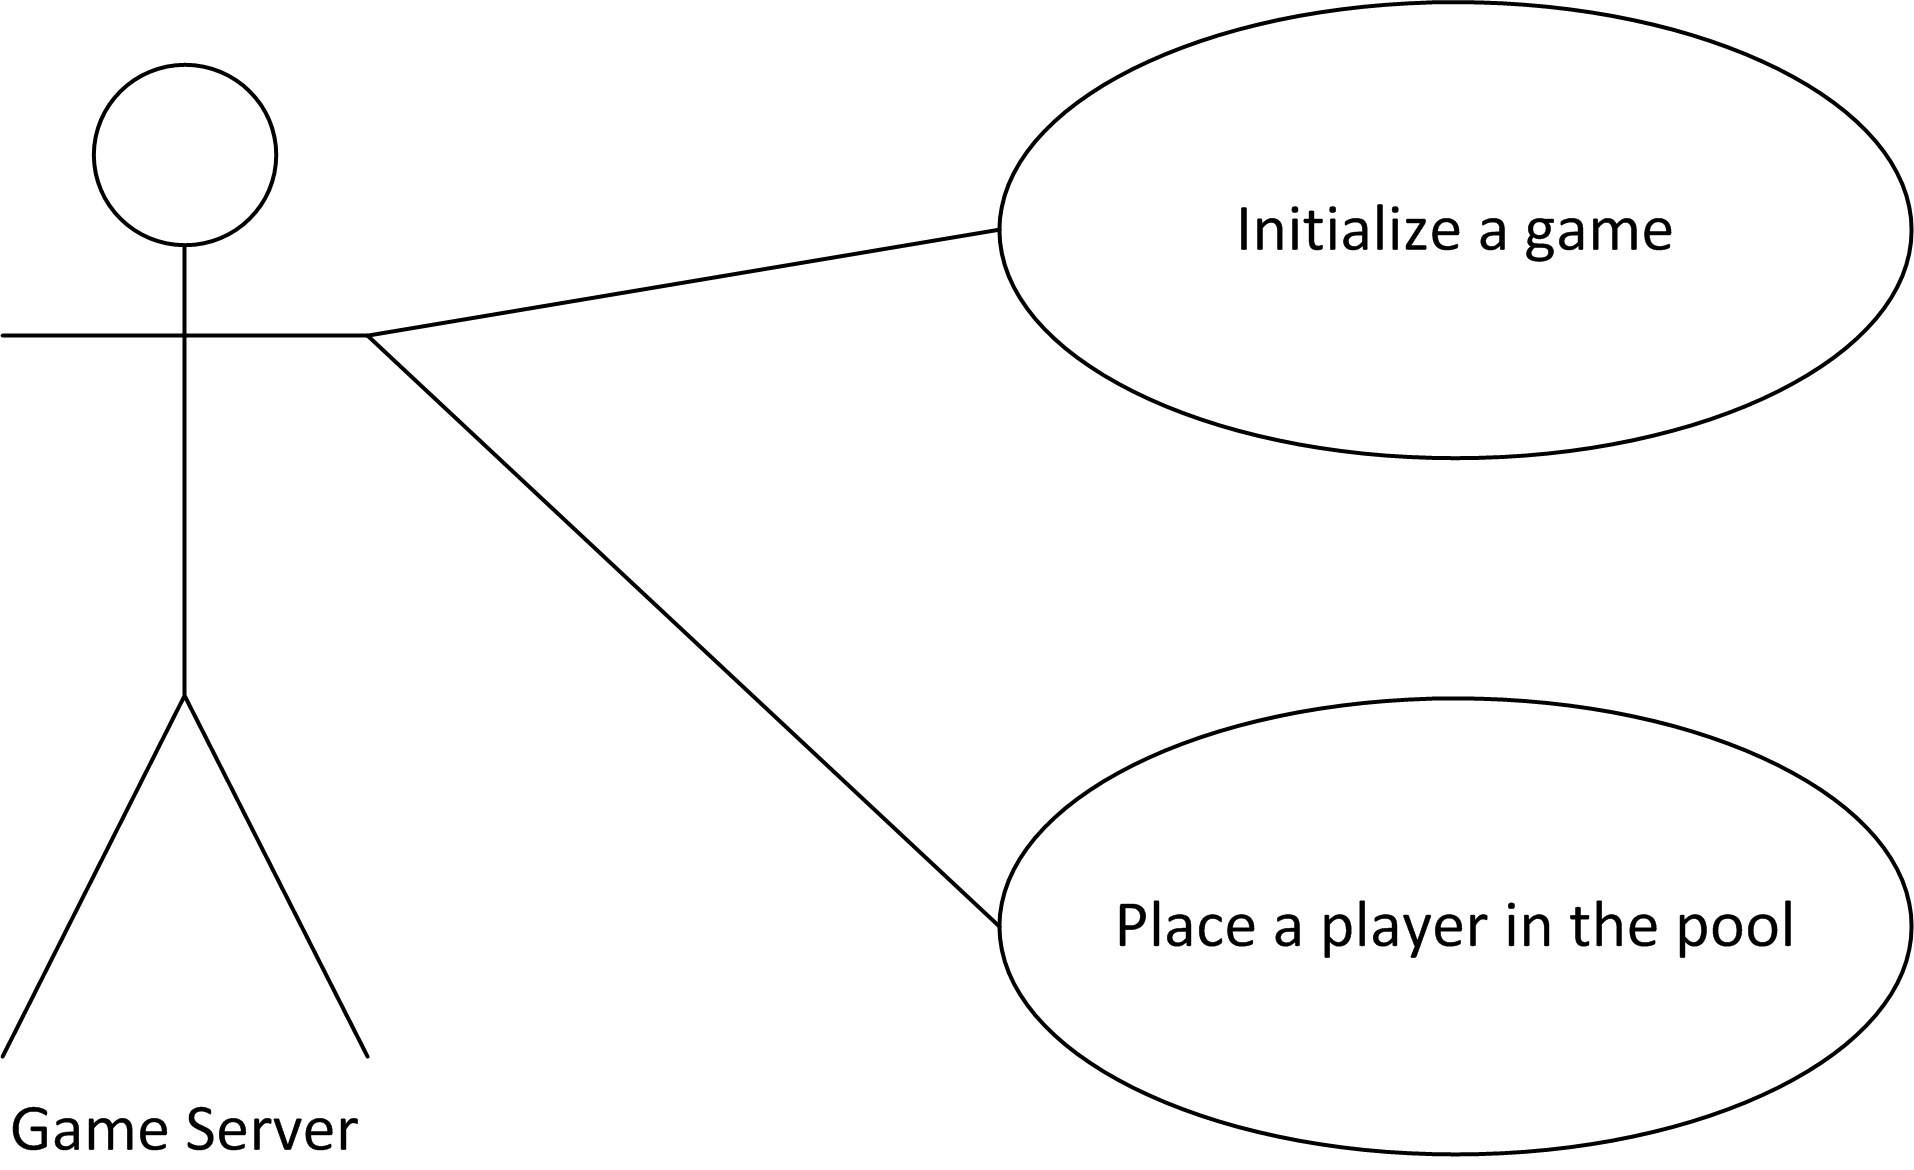
\includegraphics[scale=1.00]{UGS_usecases_gameserver.jpg}

\subsection{Person running a game client}
Actions that can be performed by a person running a game client, after successful connection to a server.

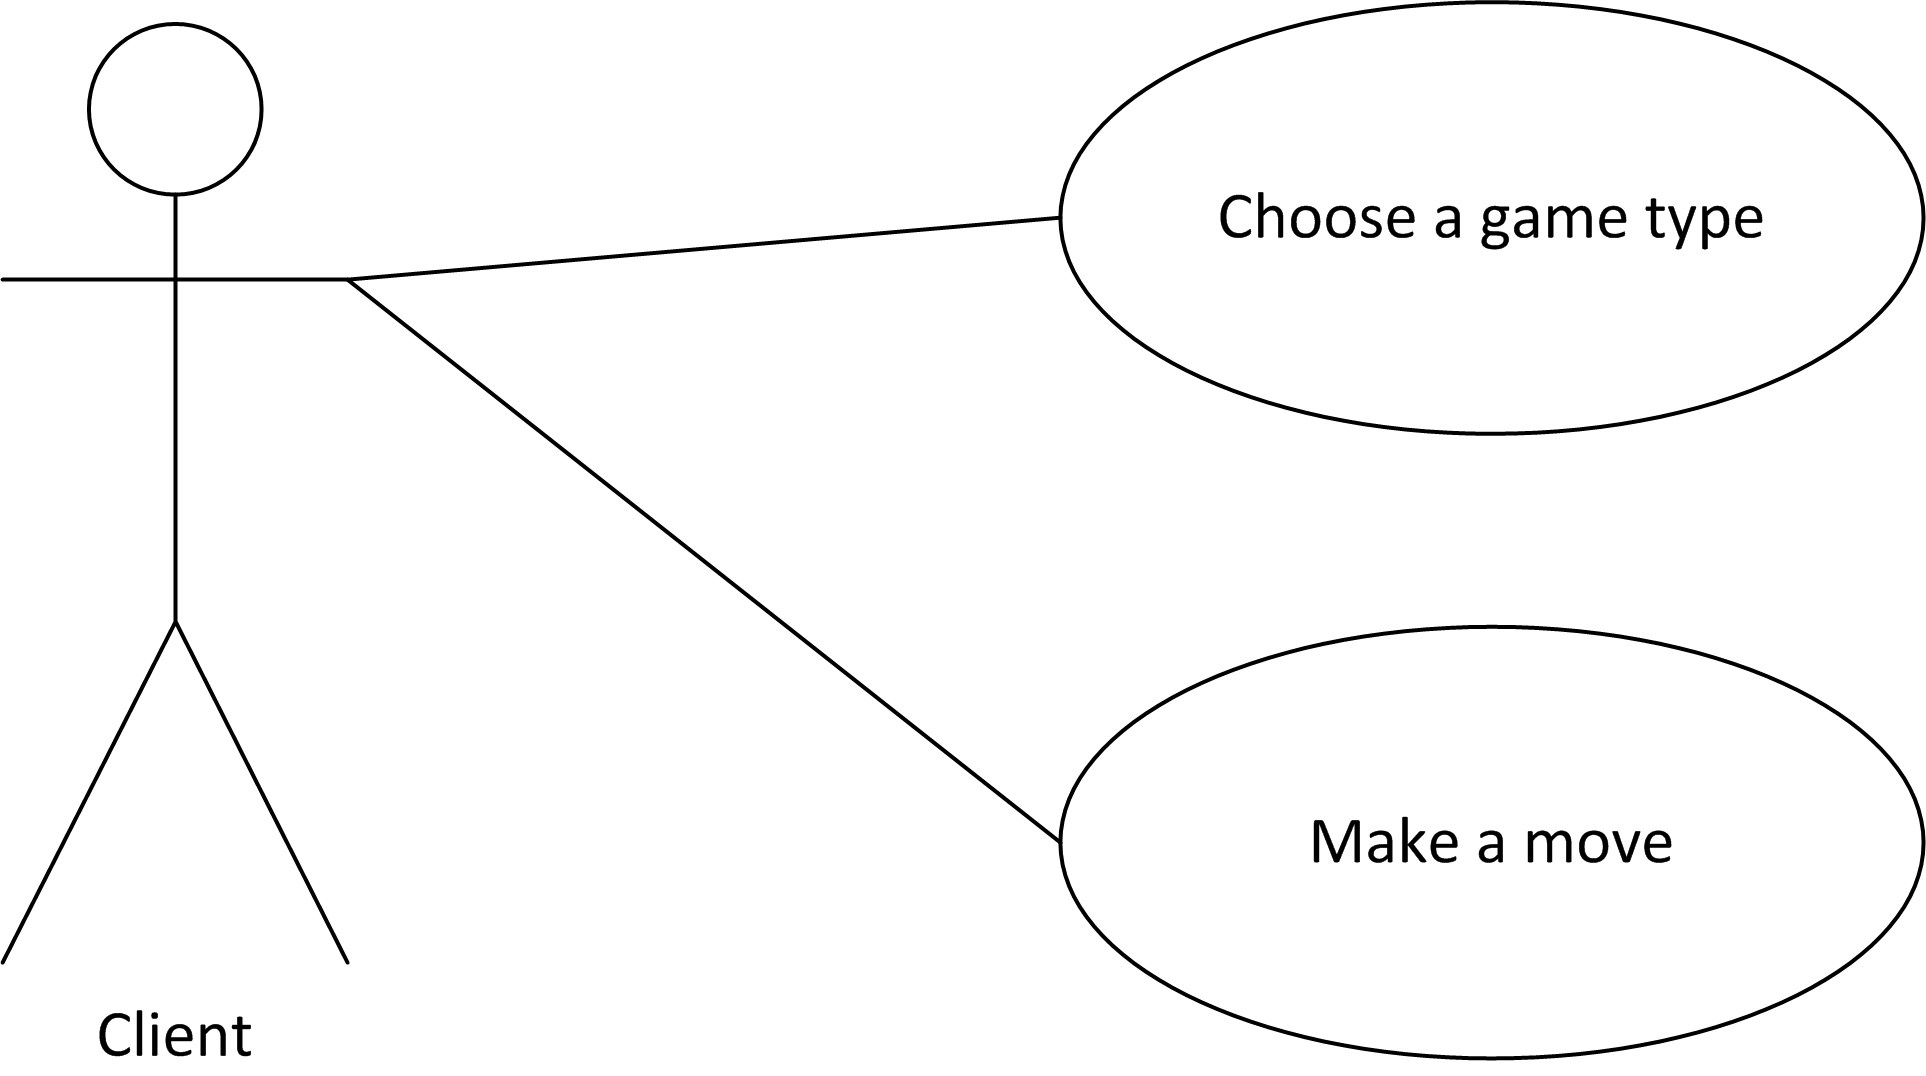
\includegraphics[scale=1.00]{UGS_usecases_client.jpg}


\pagebreak[4]


\subsection{A game client accessing and using game server}
Actions performed by all parties during the game.

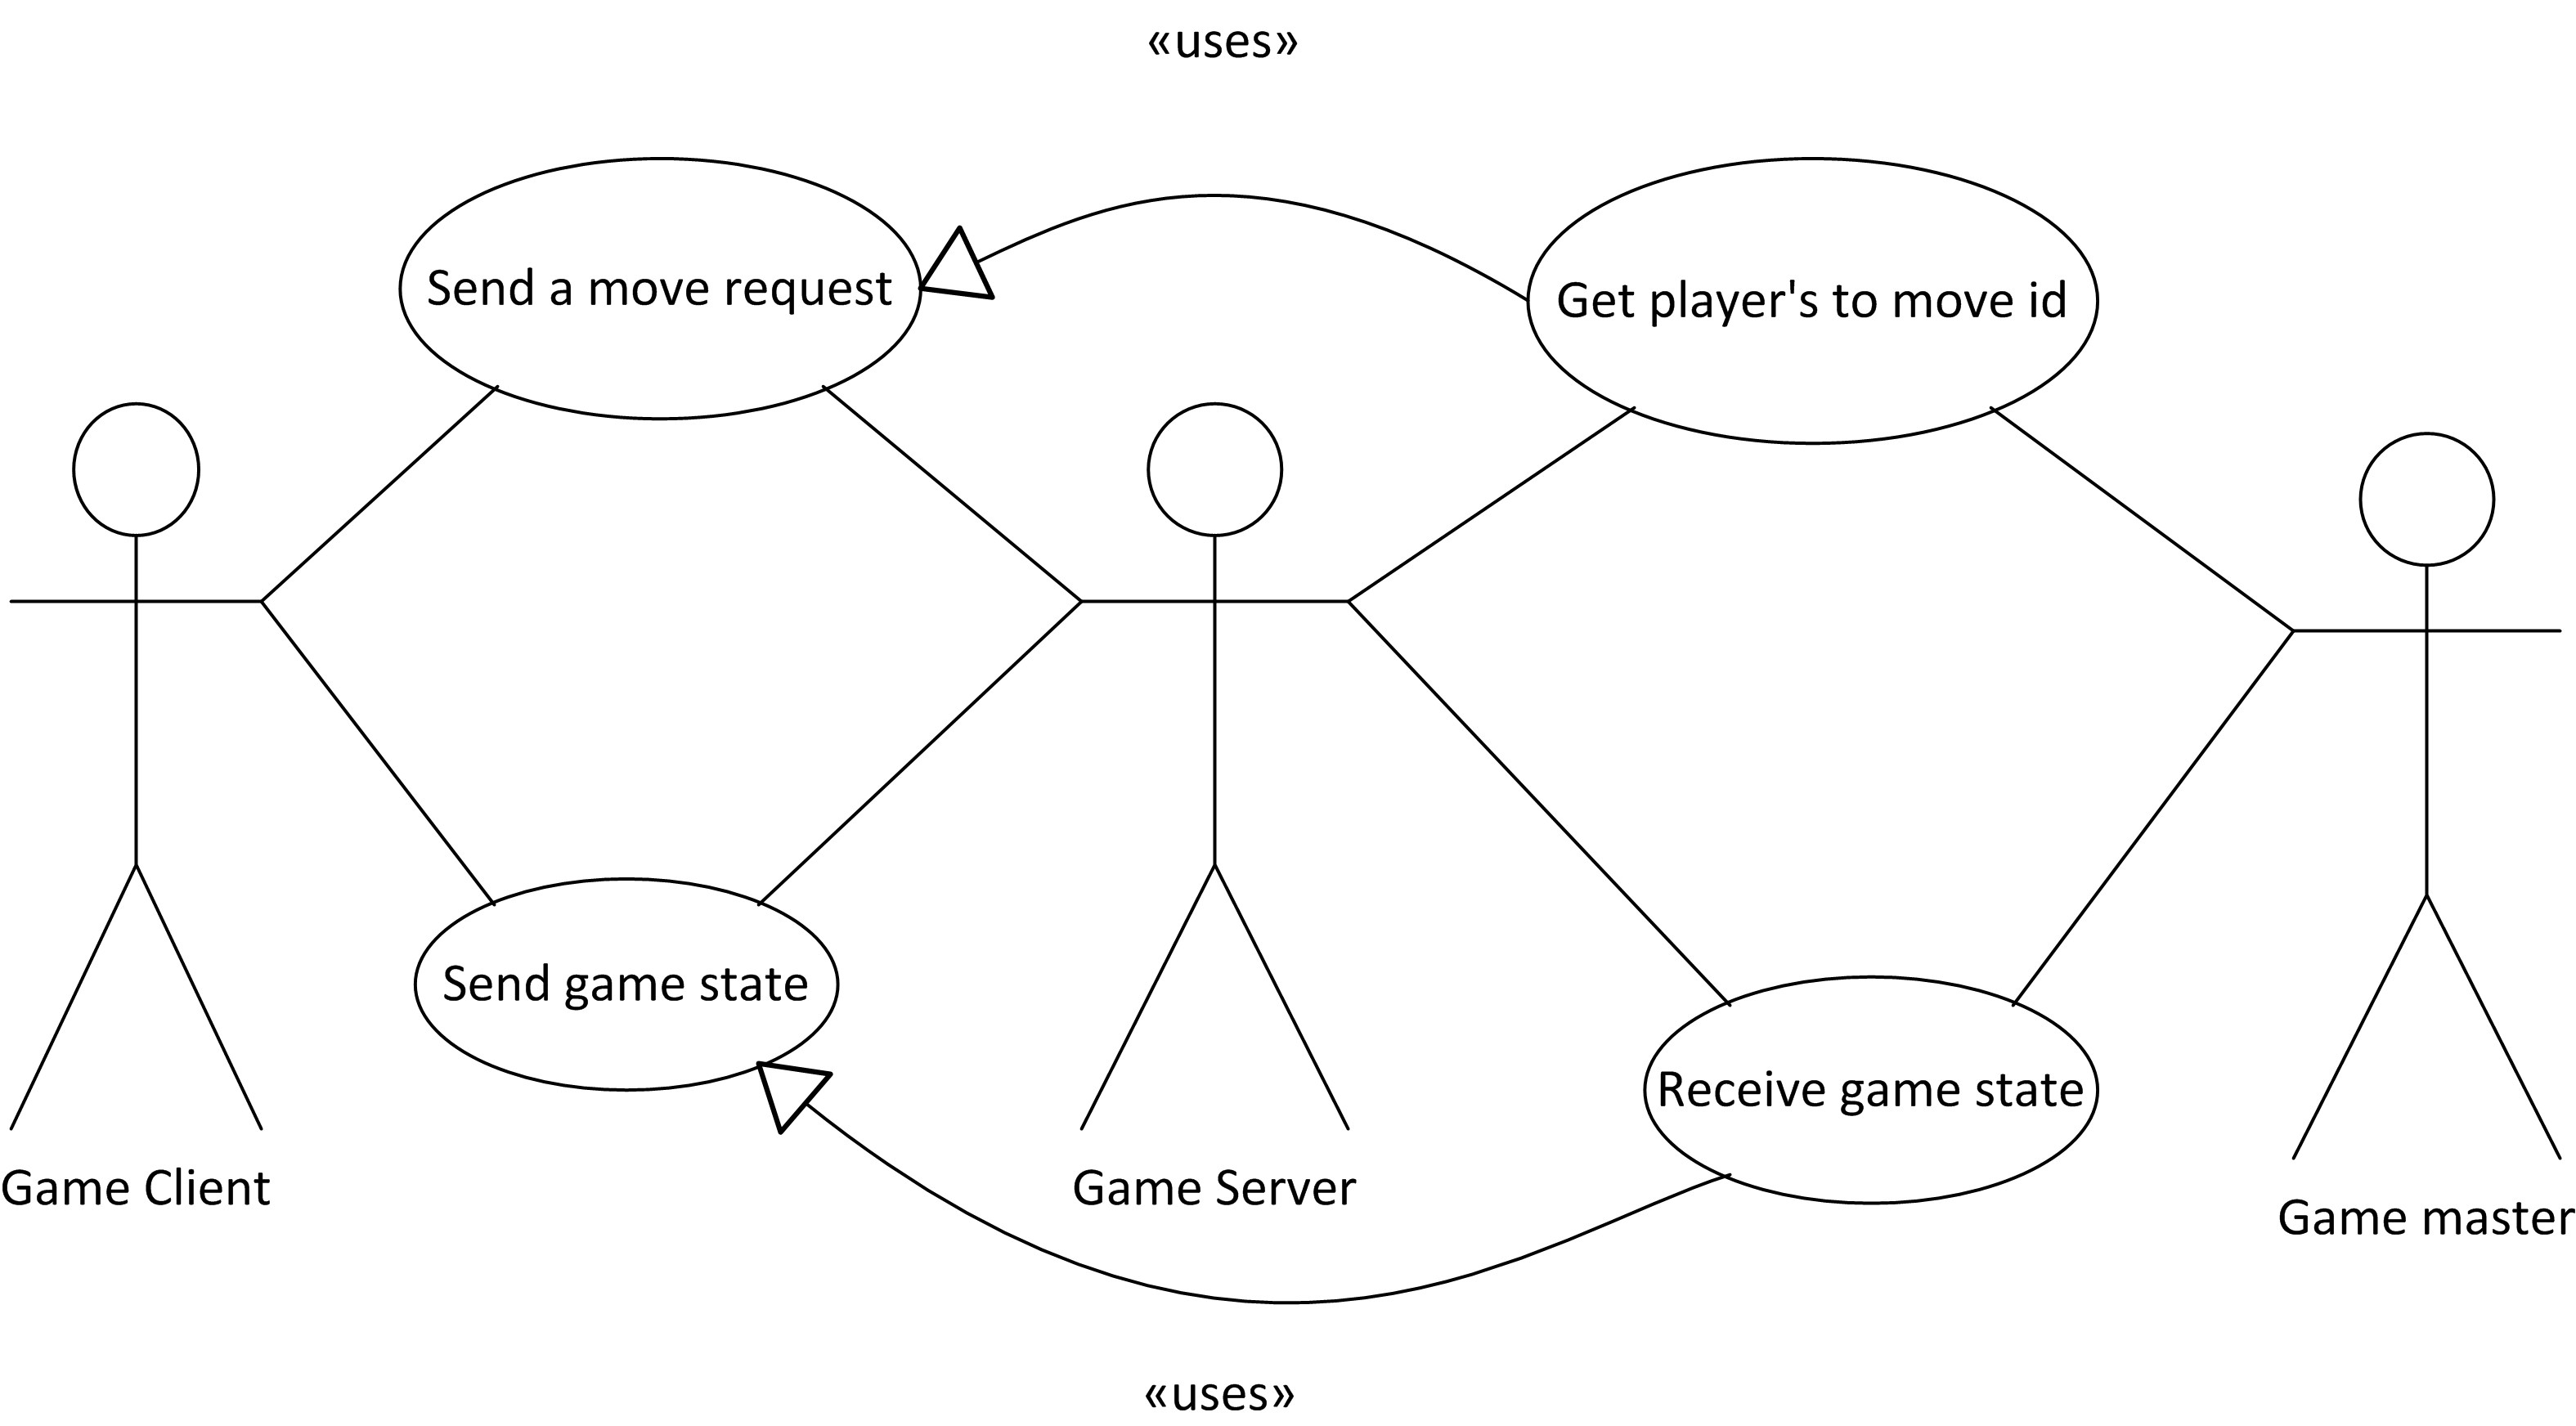
\includegraphics[scale=1.20]{UGS_usecases_application-client,server,master.jpg}

\subsection{Game server communicating with game client}
Game server communicating with game client, during the game.
 
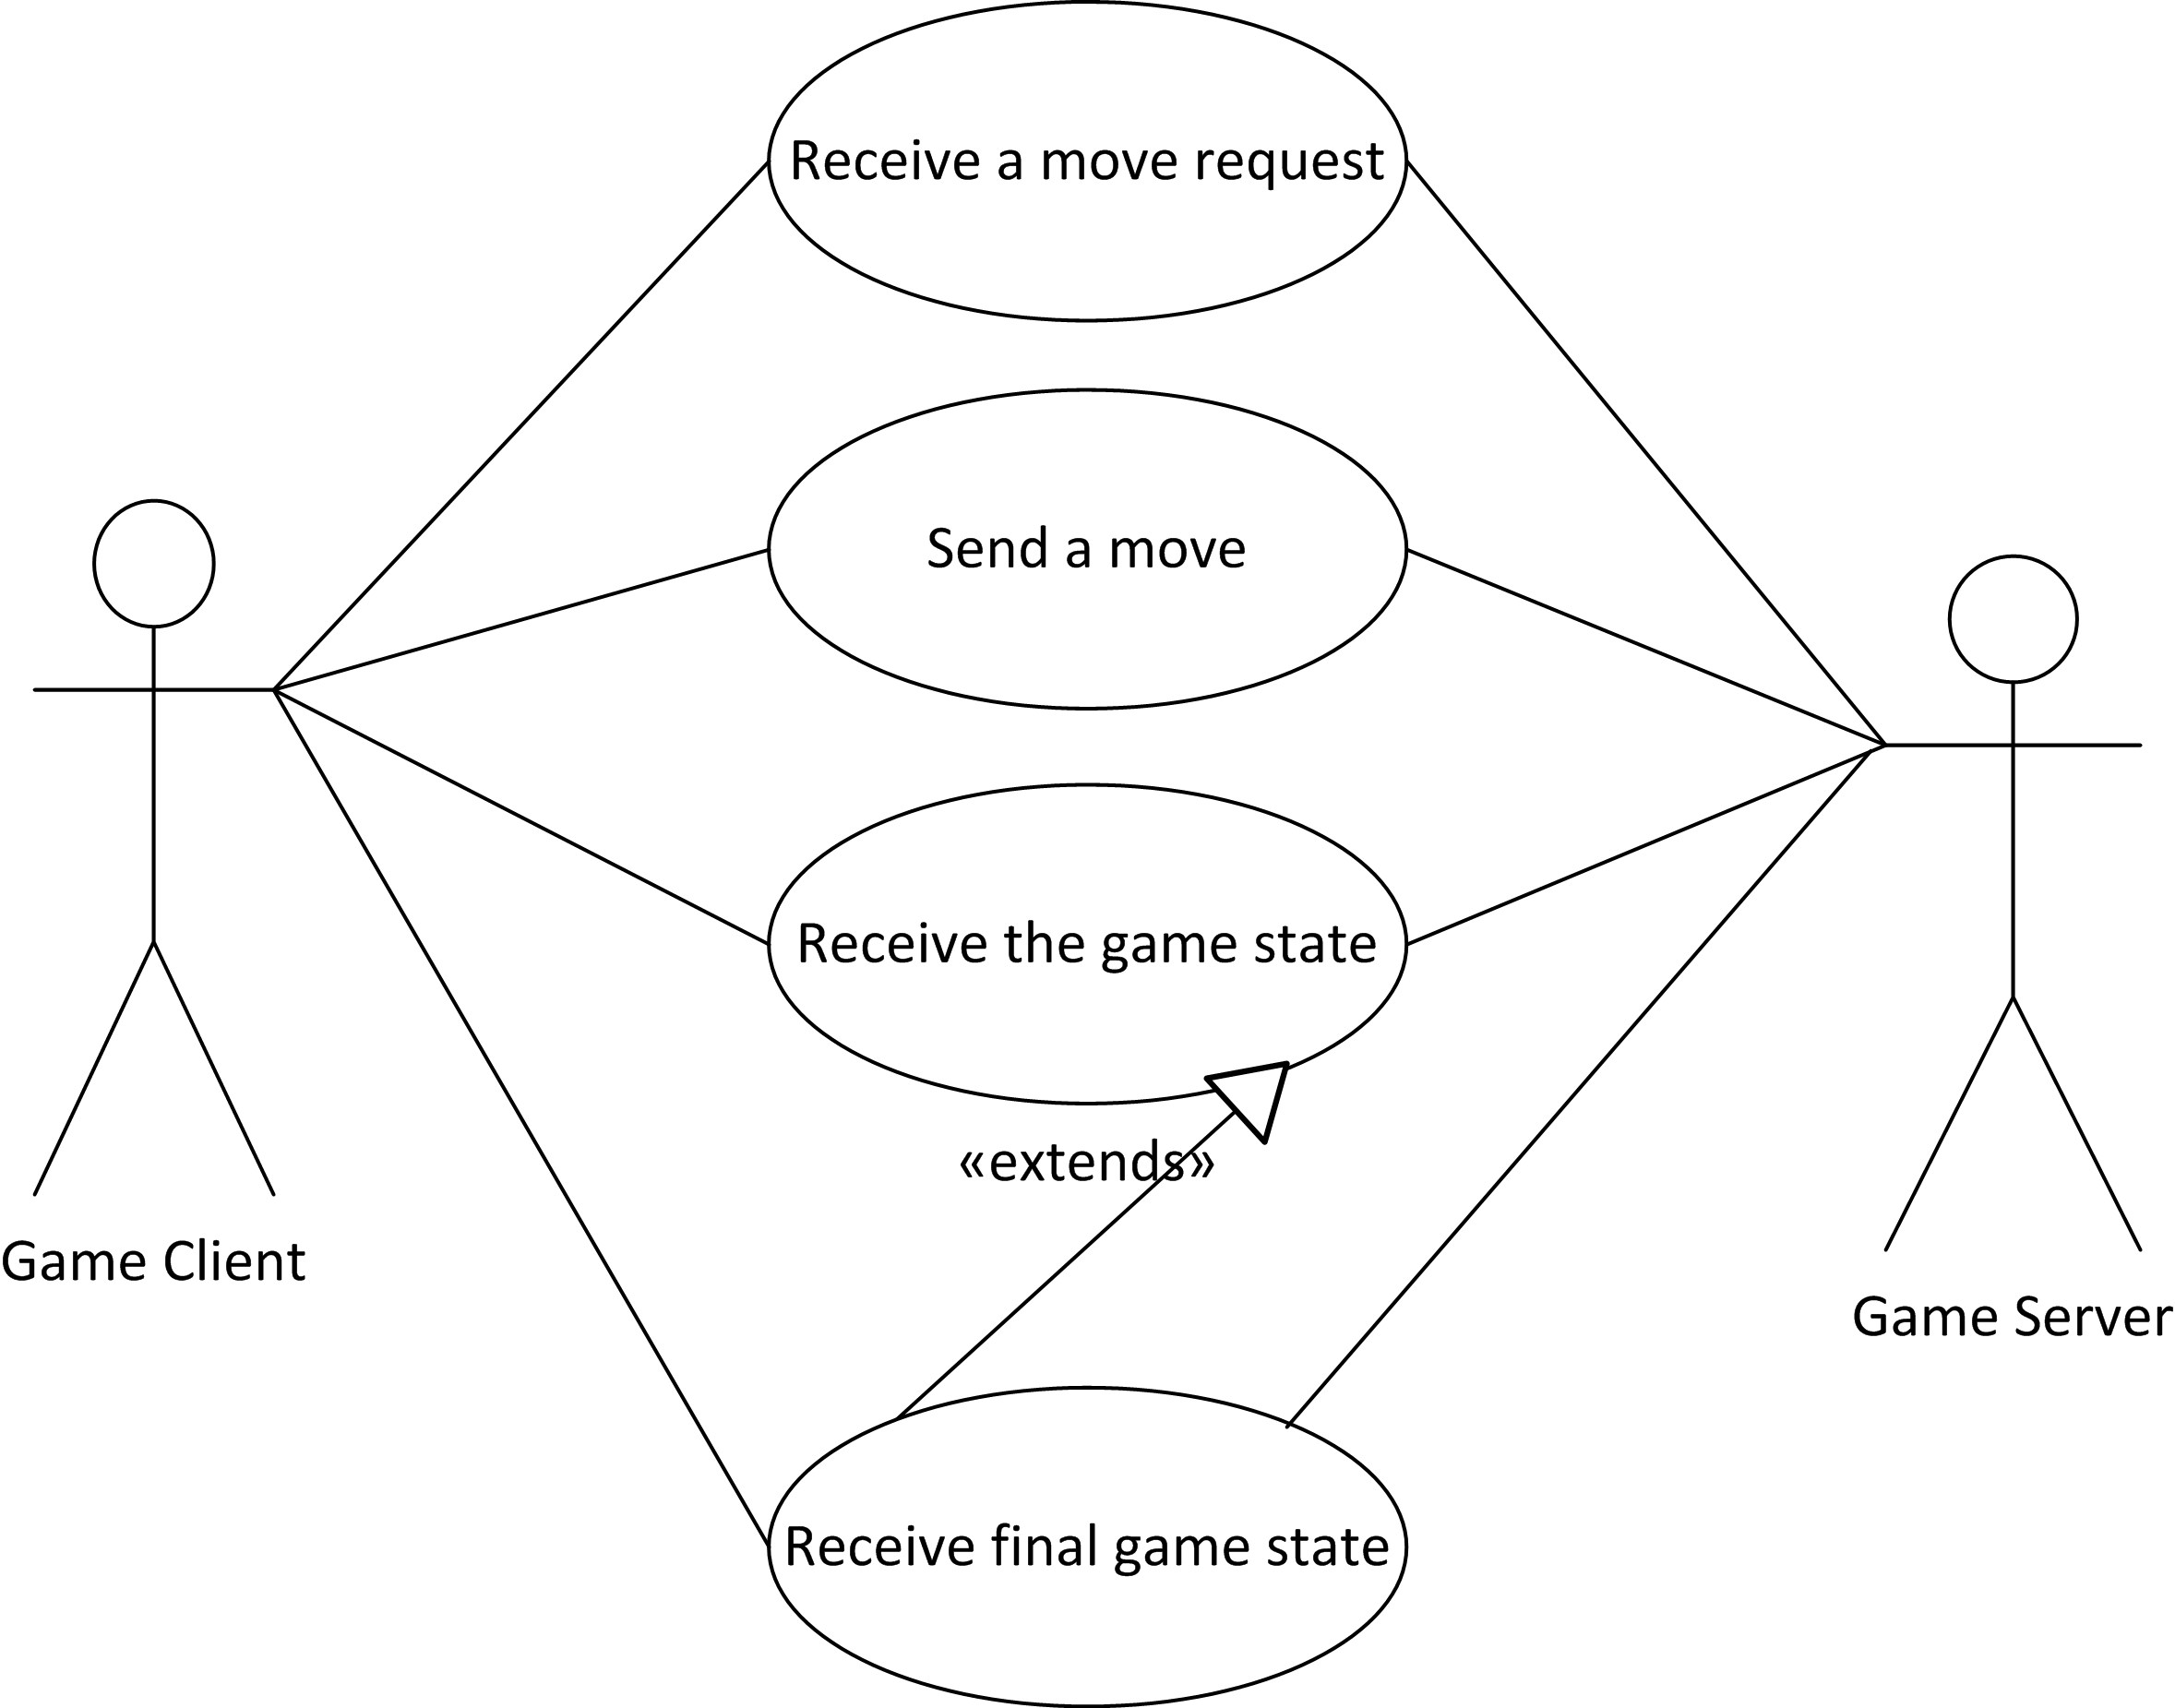
\includegraphics[scale=1.20]{UGS_usecases_application-client,server.jpg}

\section{Input data format}
Every object that can be sent between game actors is capable of being converted into XML and back, 
without any UGS-specific data loss.


\pagebreak[4]


\section{Class diagram}
GameActor is the core class of the system, because it defines the common 
characteristics of server, master and client. Class Message is also important, because it can carry 
any information between any two actors.

Game rules is the set of any relevant data that make the rules of the game, and set of operations 
that make it possible for the interested parties to check an aspect of the game such as: validity 
of the move, is the game still on or rather someone just won, constraints of the game such as time limits
for a single move, time limits for a player for a whole game, etc.

Game type contains information about kind of game, in the sense of whether the players play simultaneously 
or take turns, also whether there are teams of players in this game or not, and any other relevant information.

Game state contains current state of the game: game board, and state of each players' hands 
in case of playing cards or other similar games, list of players, and any other relevant information, 
such that there is no ambiguity about the state of the game when an actor is basing its knowledge 
only on an object of this class.

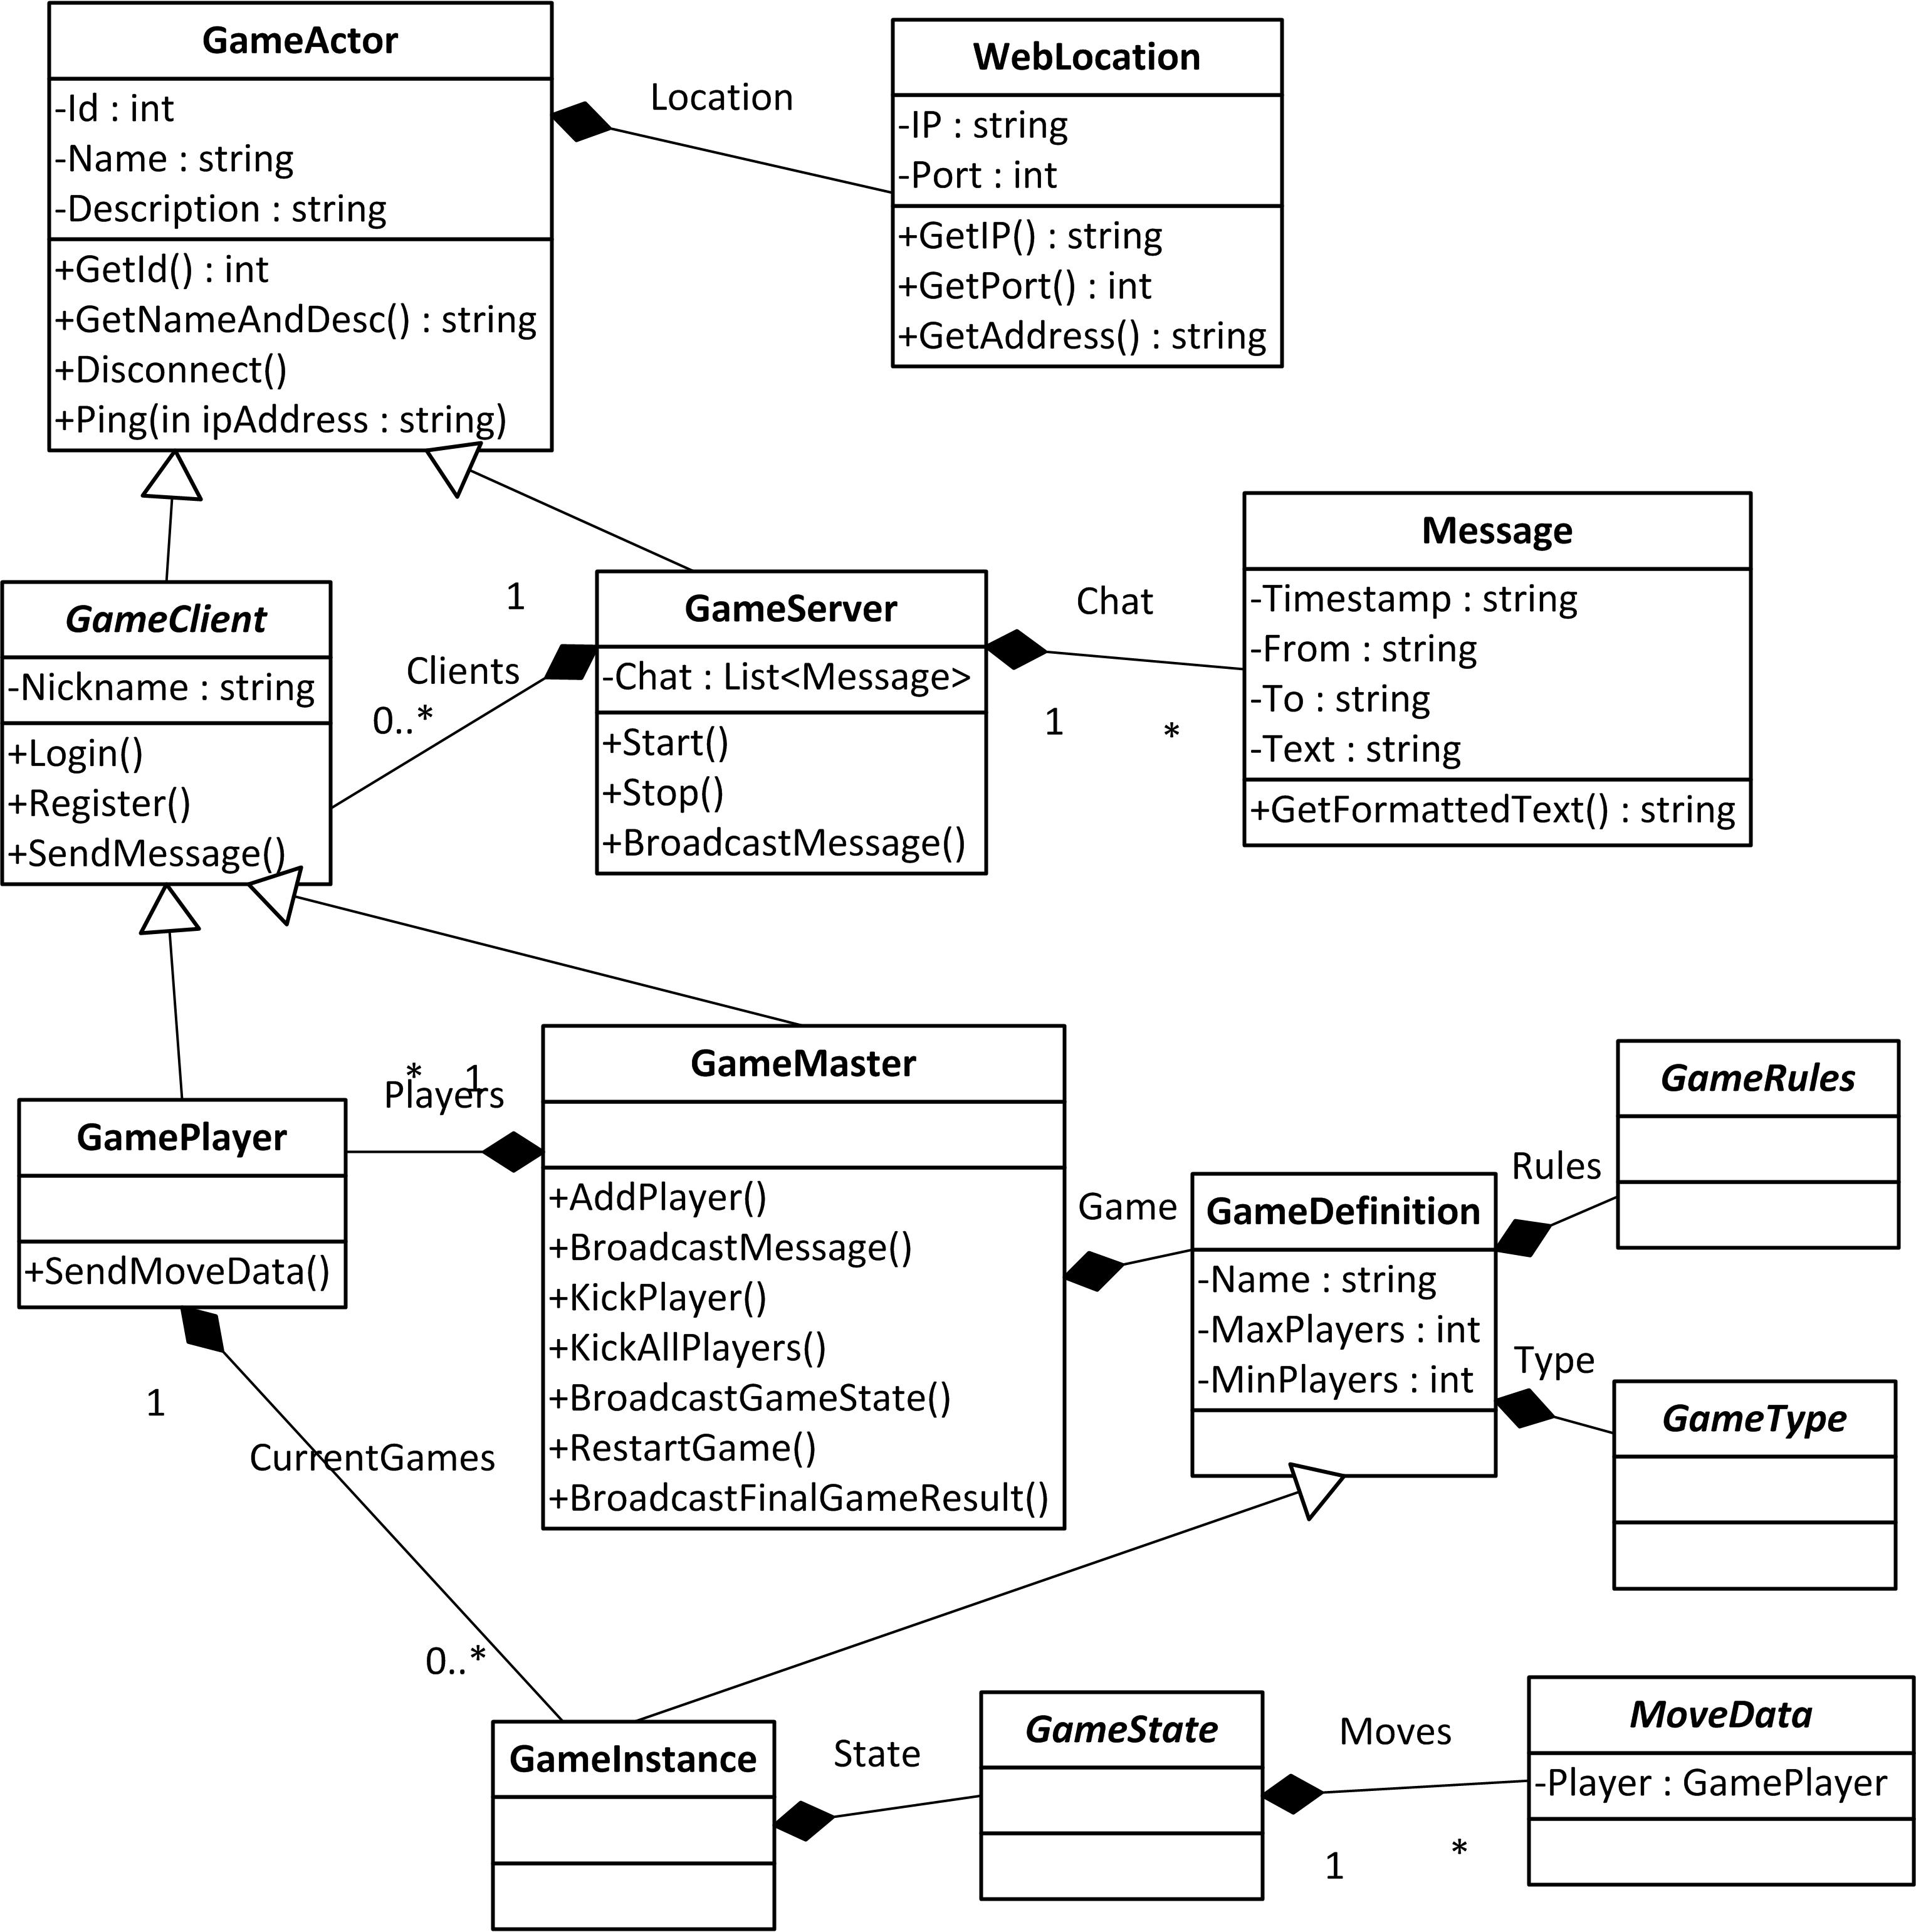
\includegraphics[scale=1.20]{UGS_classes.jpg}


\pagebreak[4]


\section{Event flow diagrams}
Interaction between game server and game applications.

\subsection{Game initialization}
Below diagram shows the events happening during game initialization process.
 
\includegraphics[scale=1.00]{UGS_events_Game_initilalization.jpg}

\subsection{Game finalization}
That is how the game will be finalized.
 
\includegraphics[scale=1.00]{UGS_events_Game_finalization.jpg}


\pagebreak[4]


\subsection{Client-server communication}
Complete view on client server communication.

\includegraphics[scale=1.00]{UGS_events_Client-server_communication.jpg}

\subsection{Master-server-player interaction}
Complete view on how the game master will communicate with game clients via the game server.

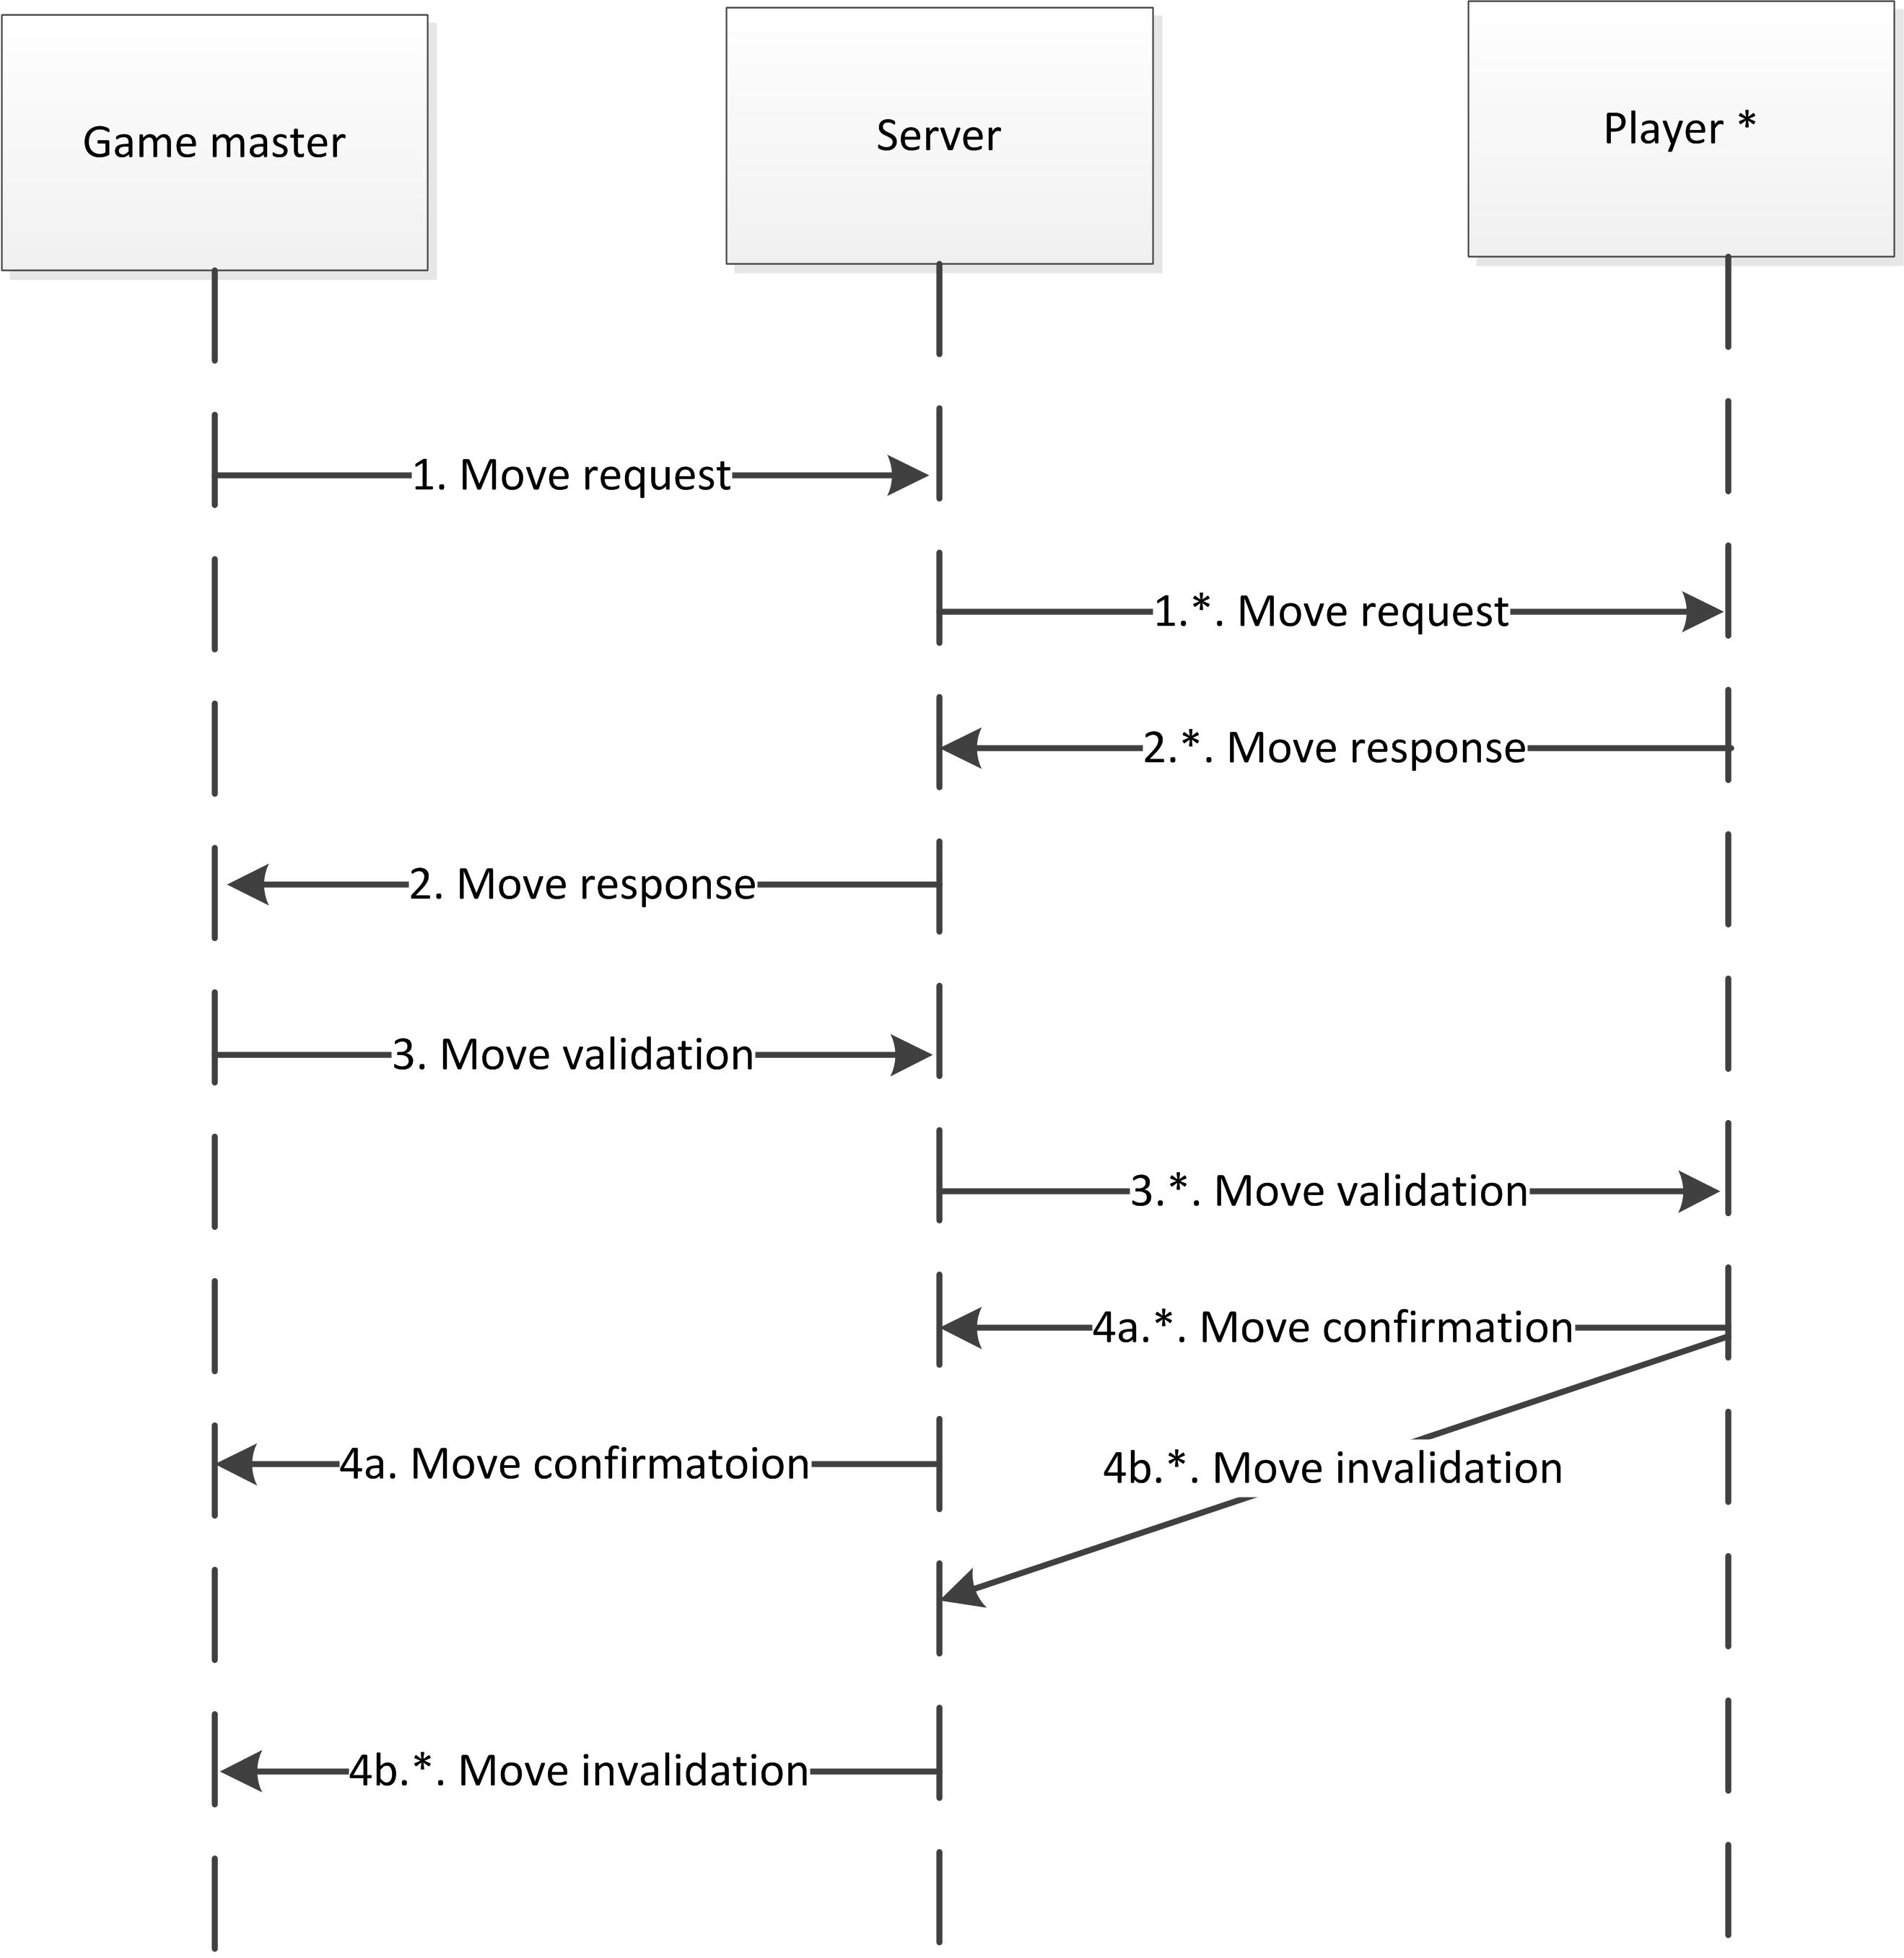
\includegraphics[scale=1.00]{UGS_events_master-server-player_interaction.jpg}


\pagebreak[4]


\section{State diagrams}

%\subsection{Client-server communication}
%Text text text\ldots

%\includegraphics[scale=1.00]{UGS_states_cielnt-server_communication.jpg}

\subsection{Game master}
List of states of the game master. At the beginning the game master is started, and is waiting for requests.

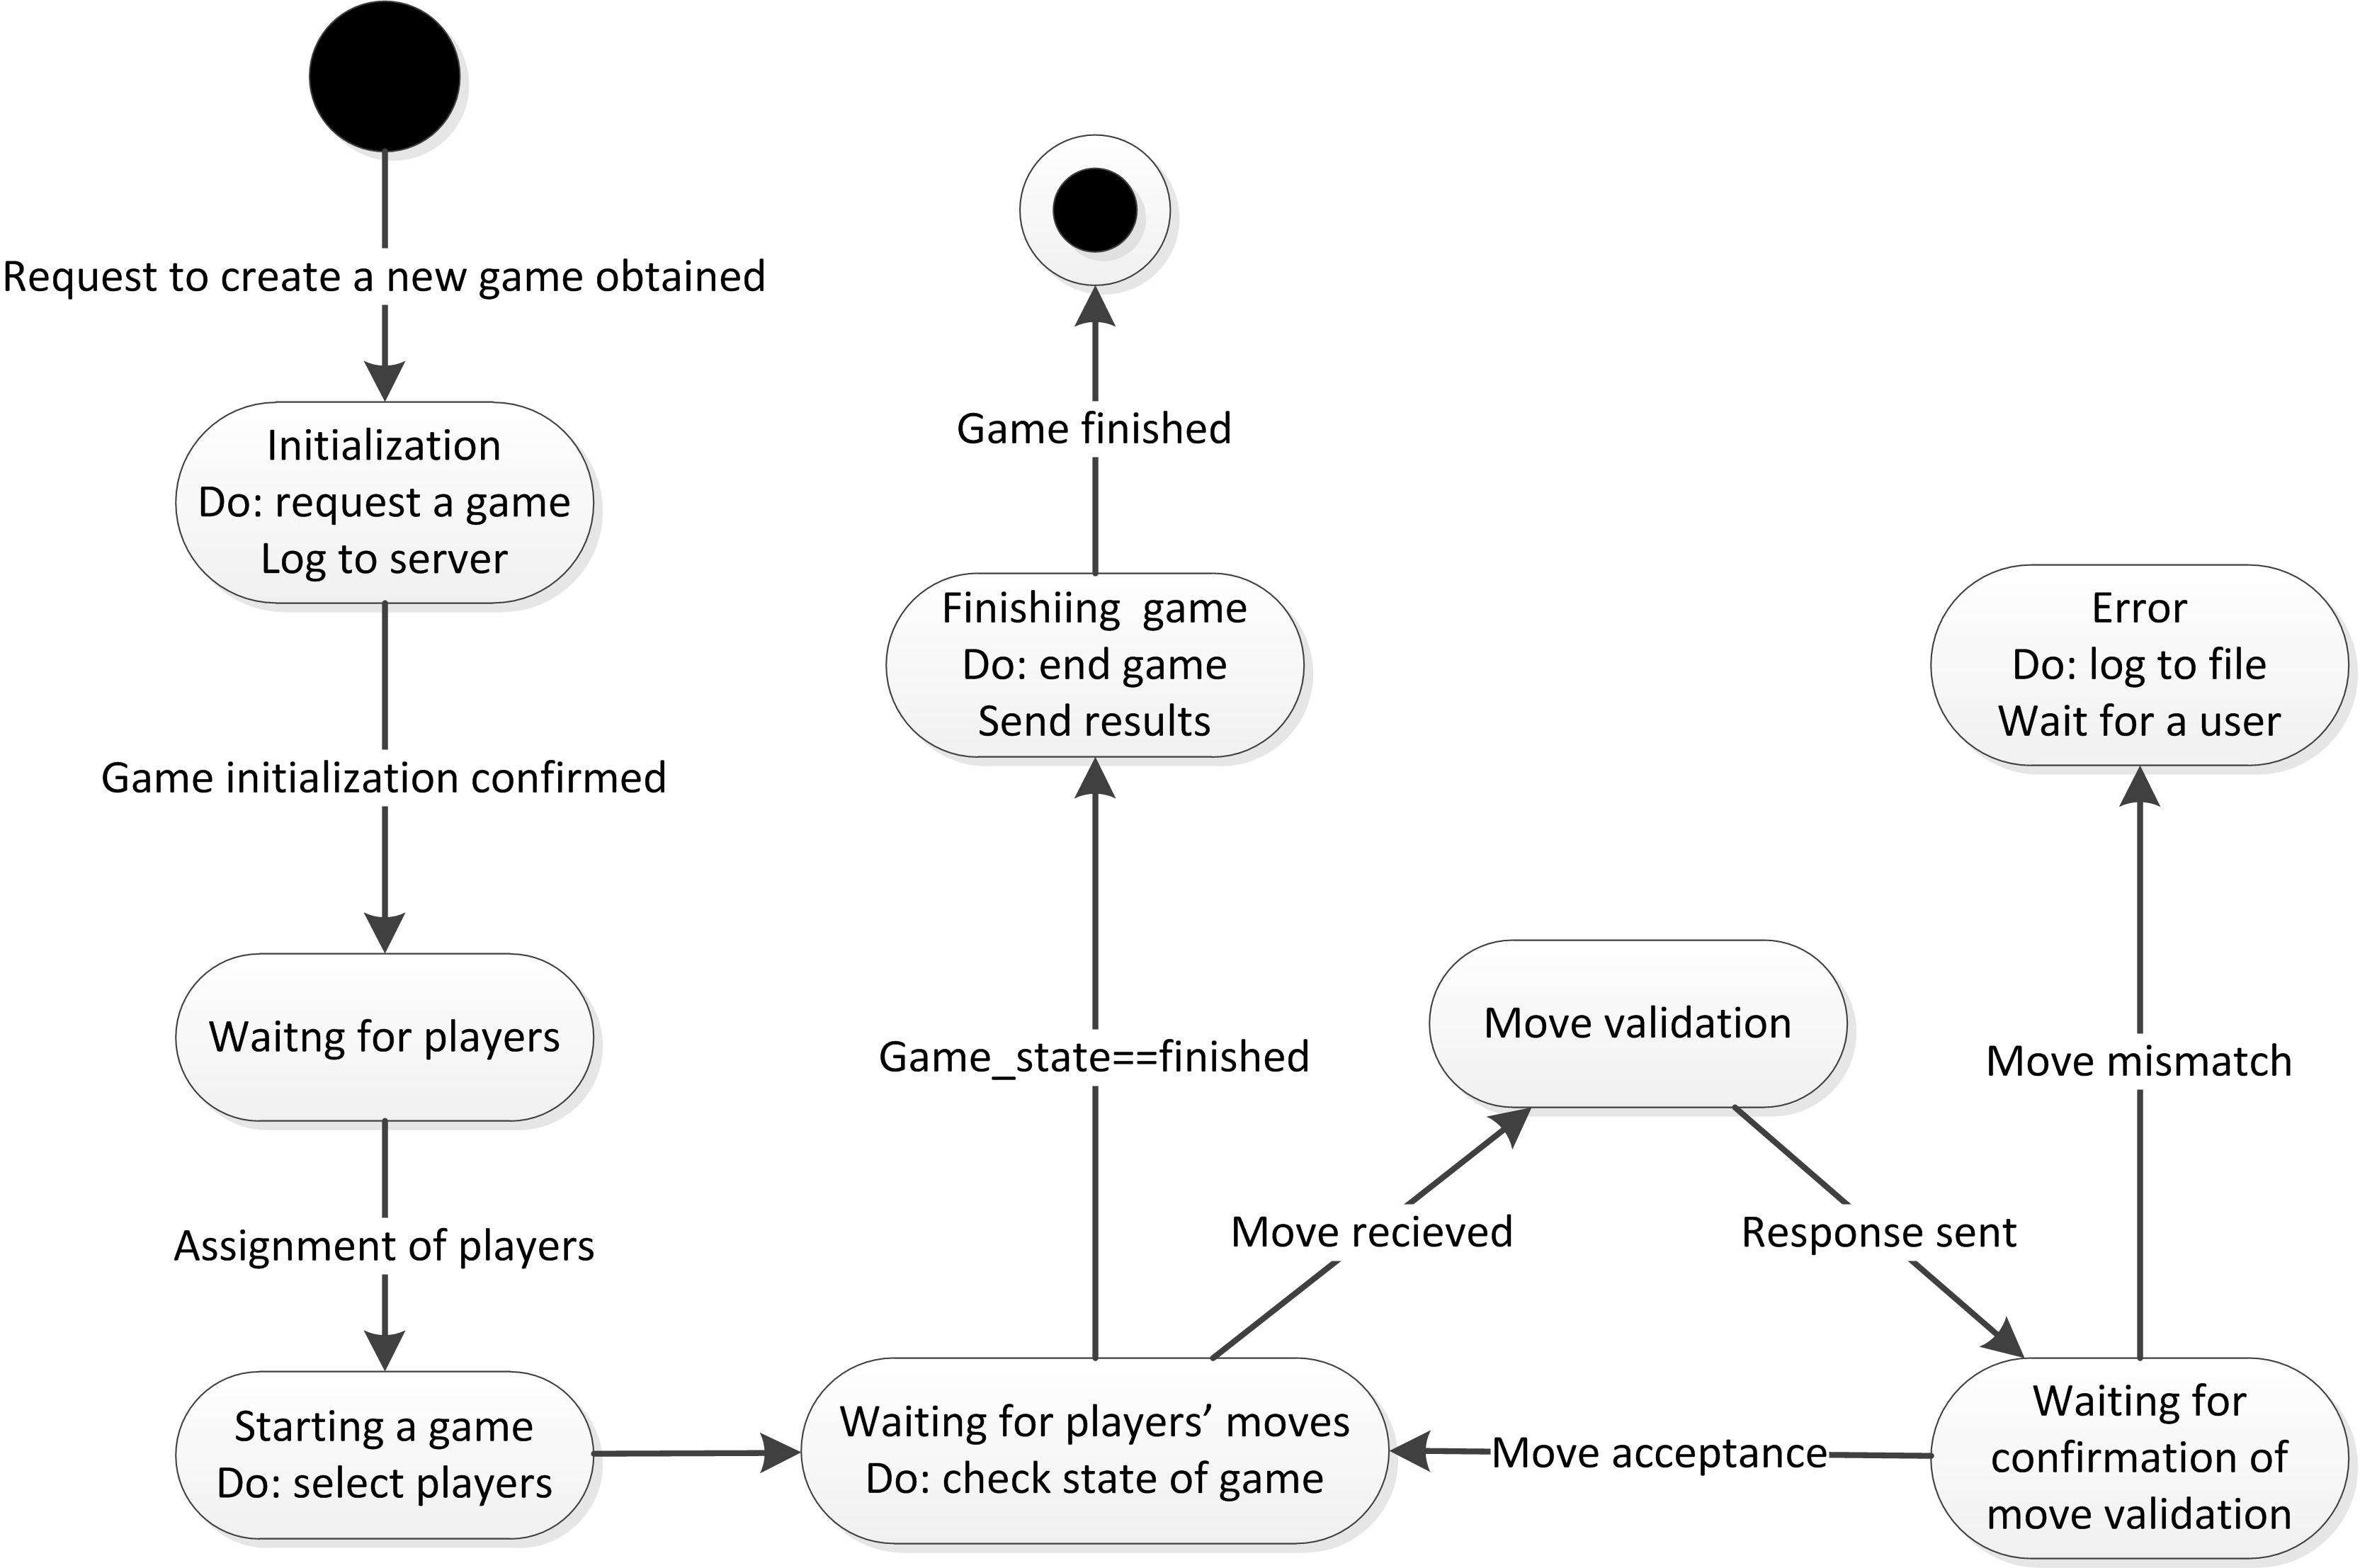
\includegraphics[scale=1.10]{UGS_states_game_master.jpg}

\subsection{Player-game}

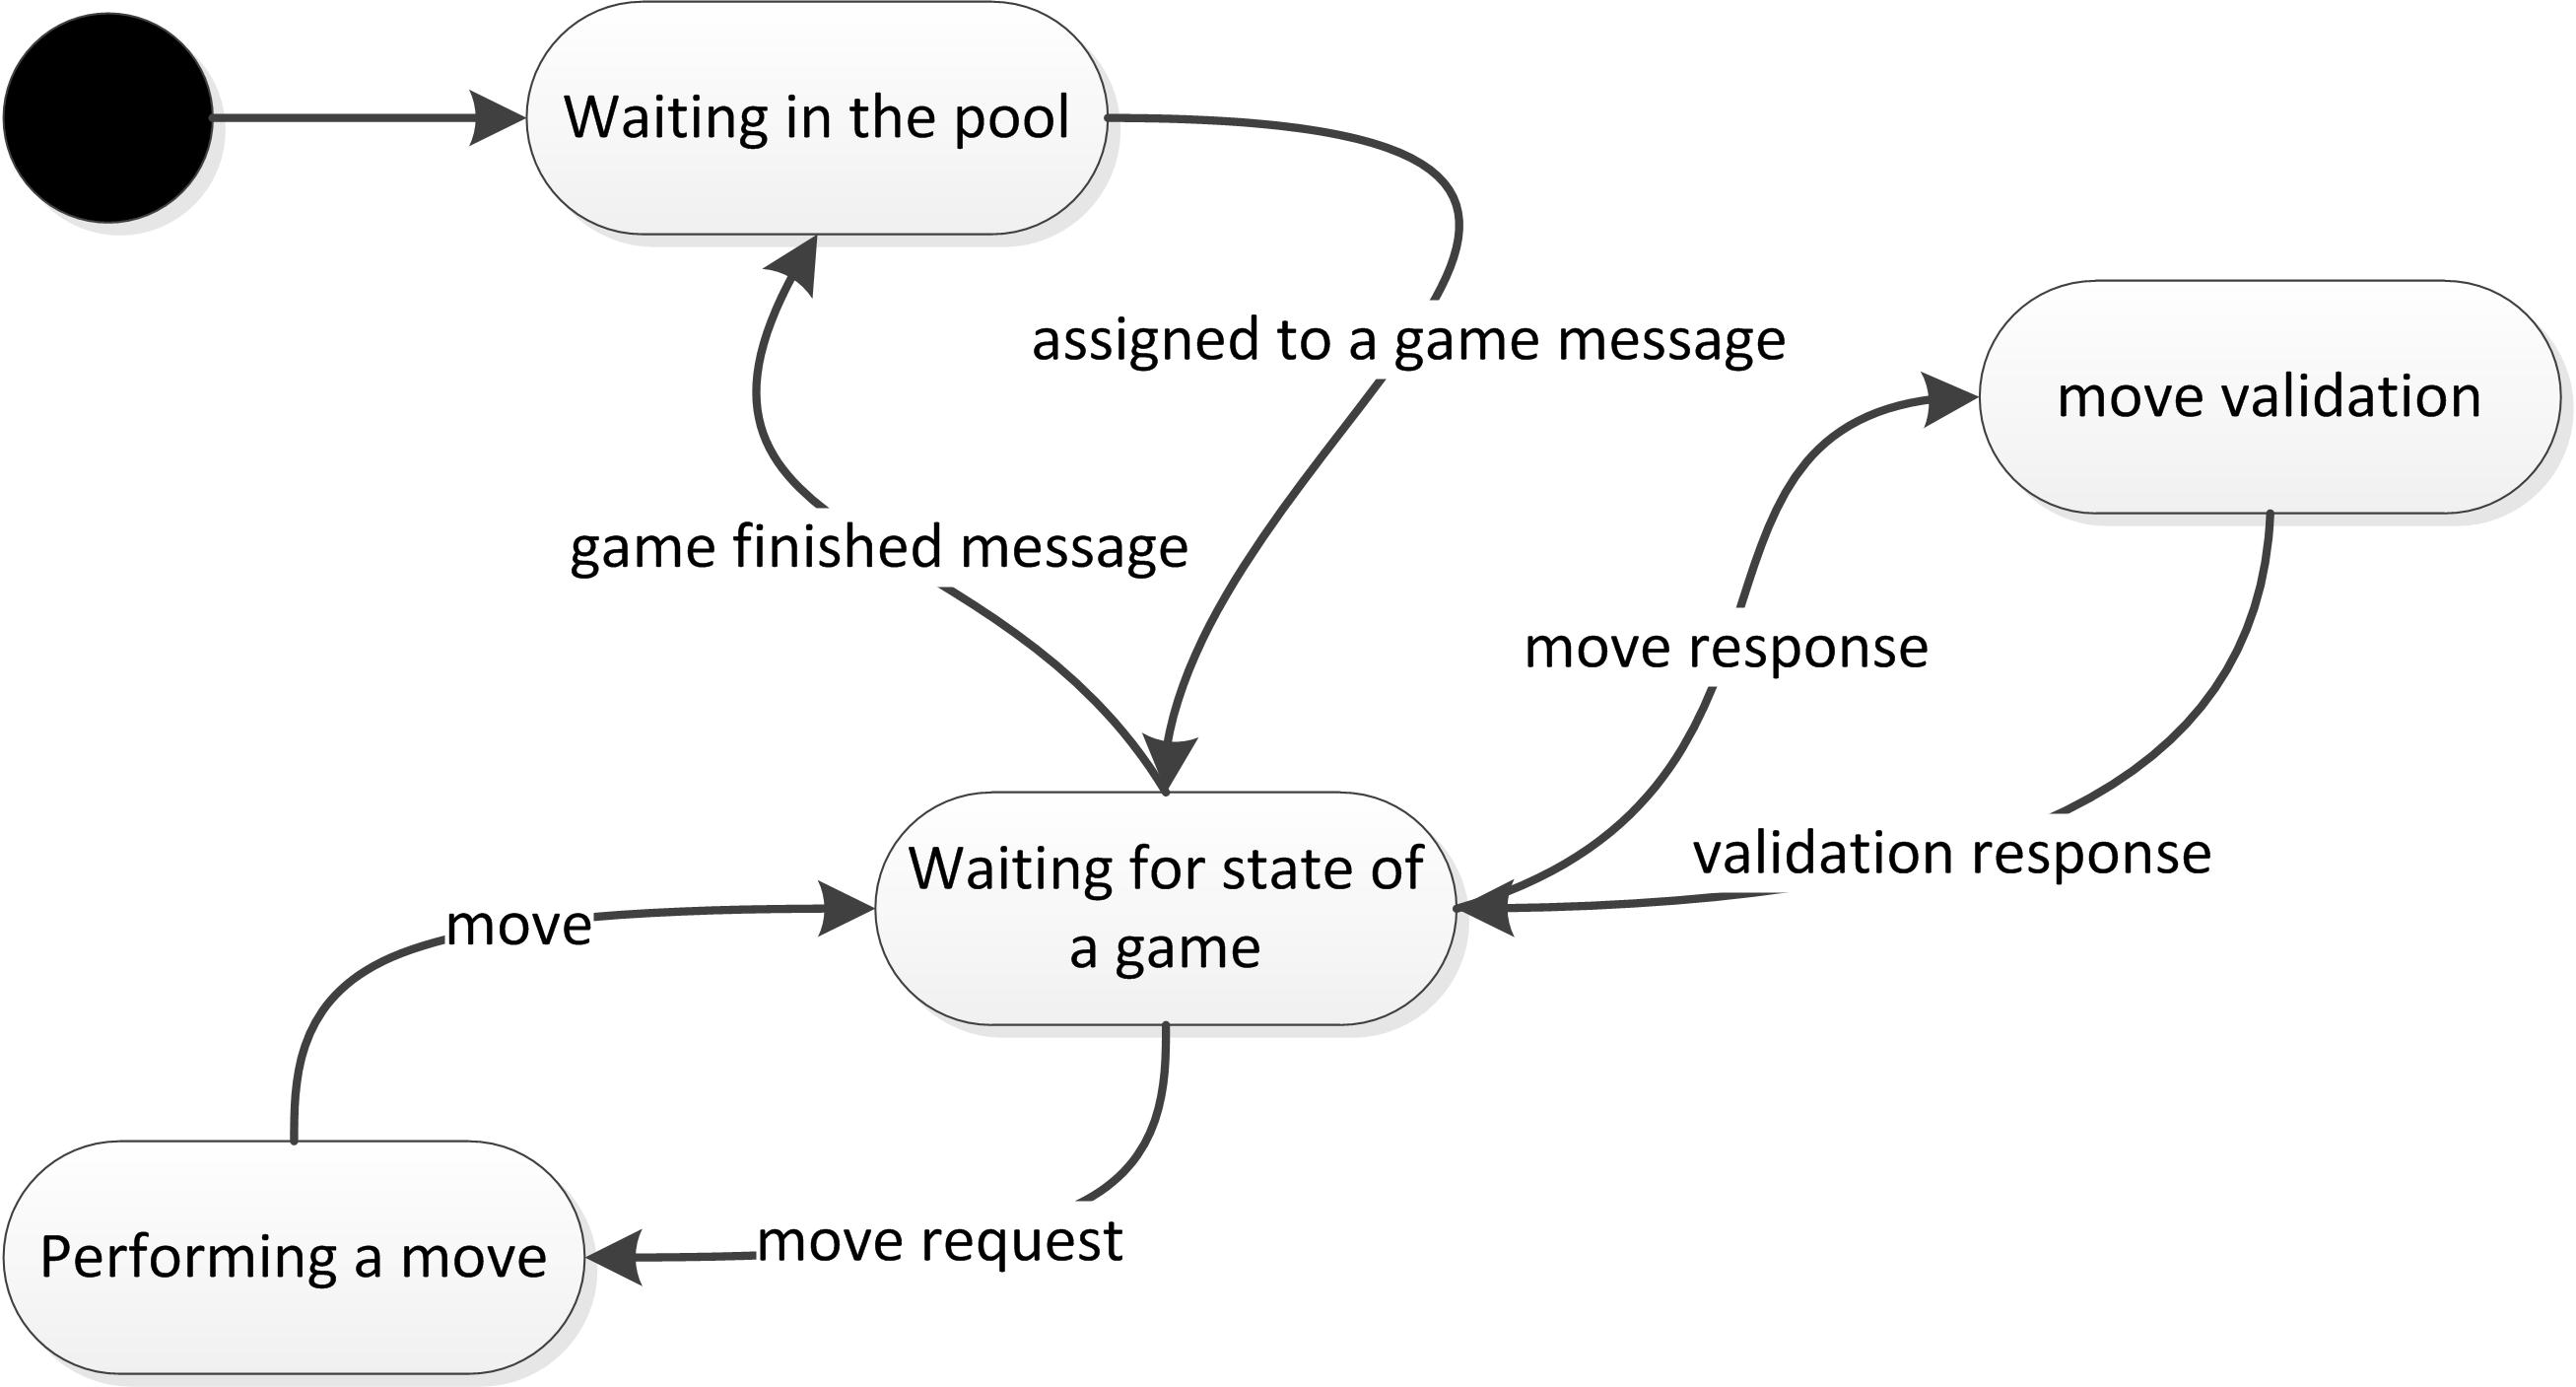
\includegraphics[scale=1.10]{UGS_states_player-game.jpg}


\pagebreak[4]


\subsection{Server}

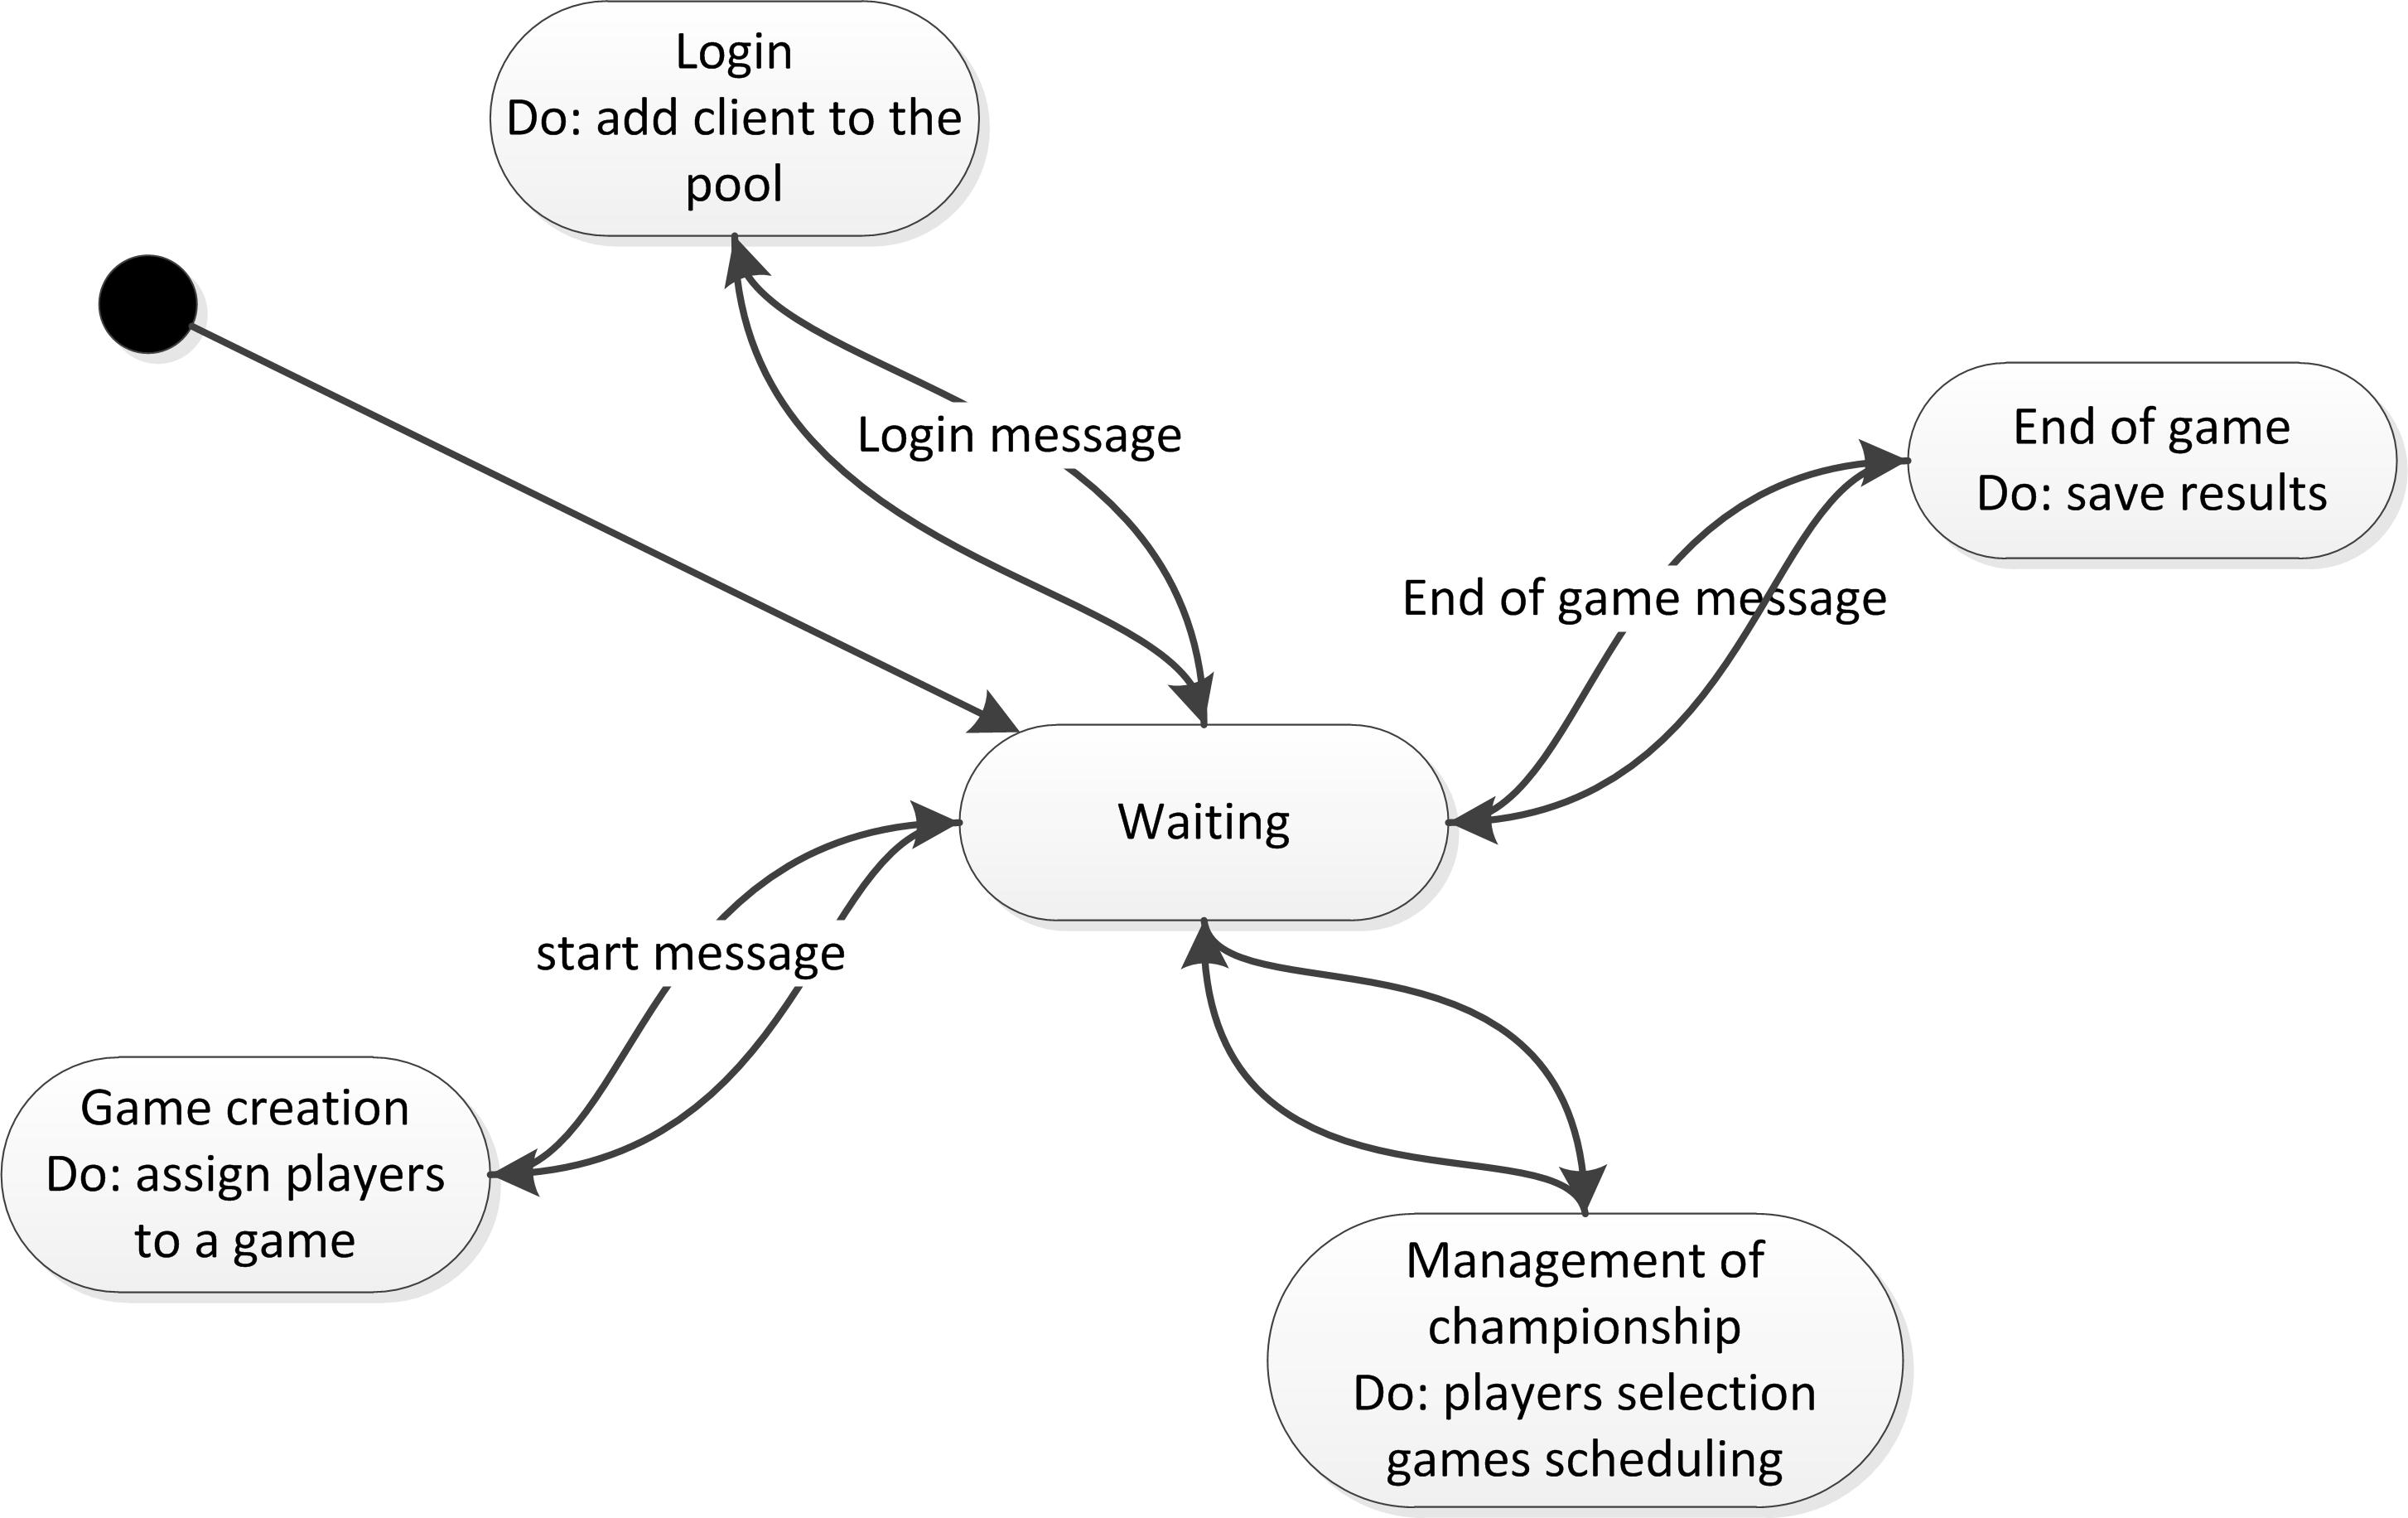
\includegraphics[scale=1.10]{UGS_states_server.jpg}

\section{Activity diagrams}

\subsection{Championship management}

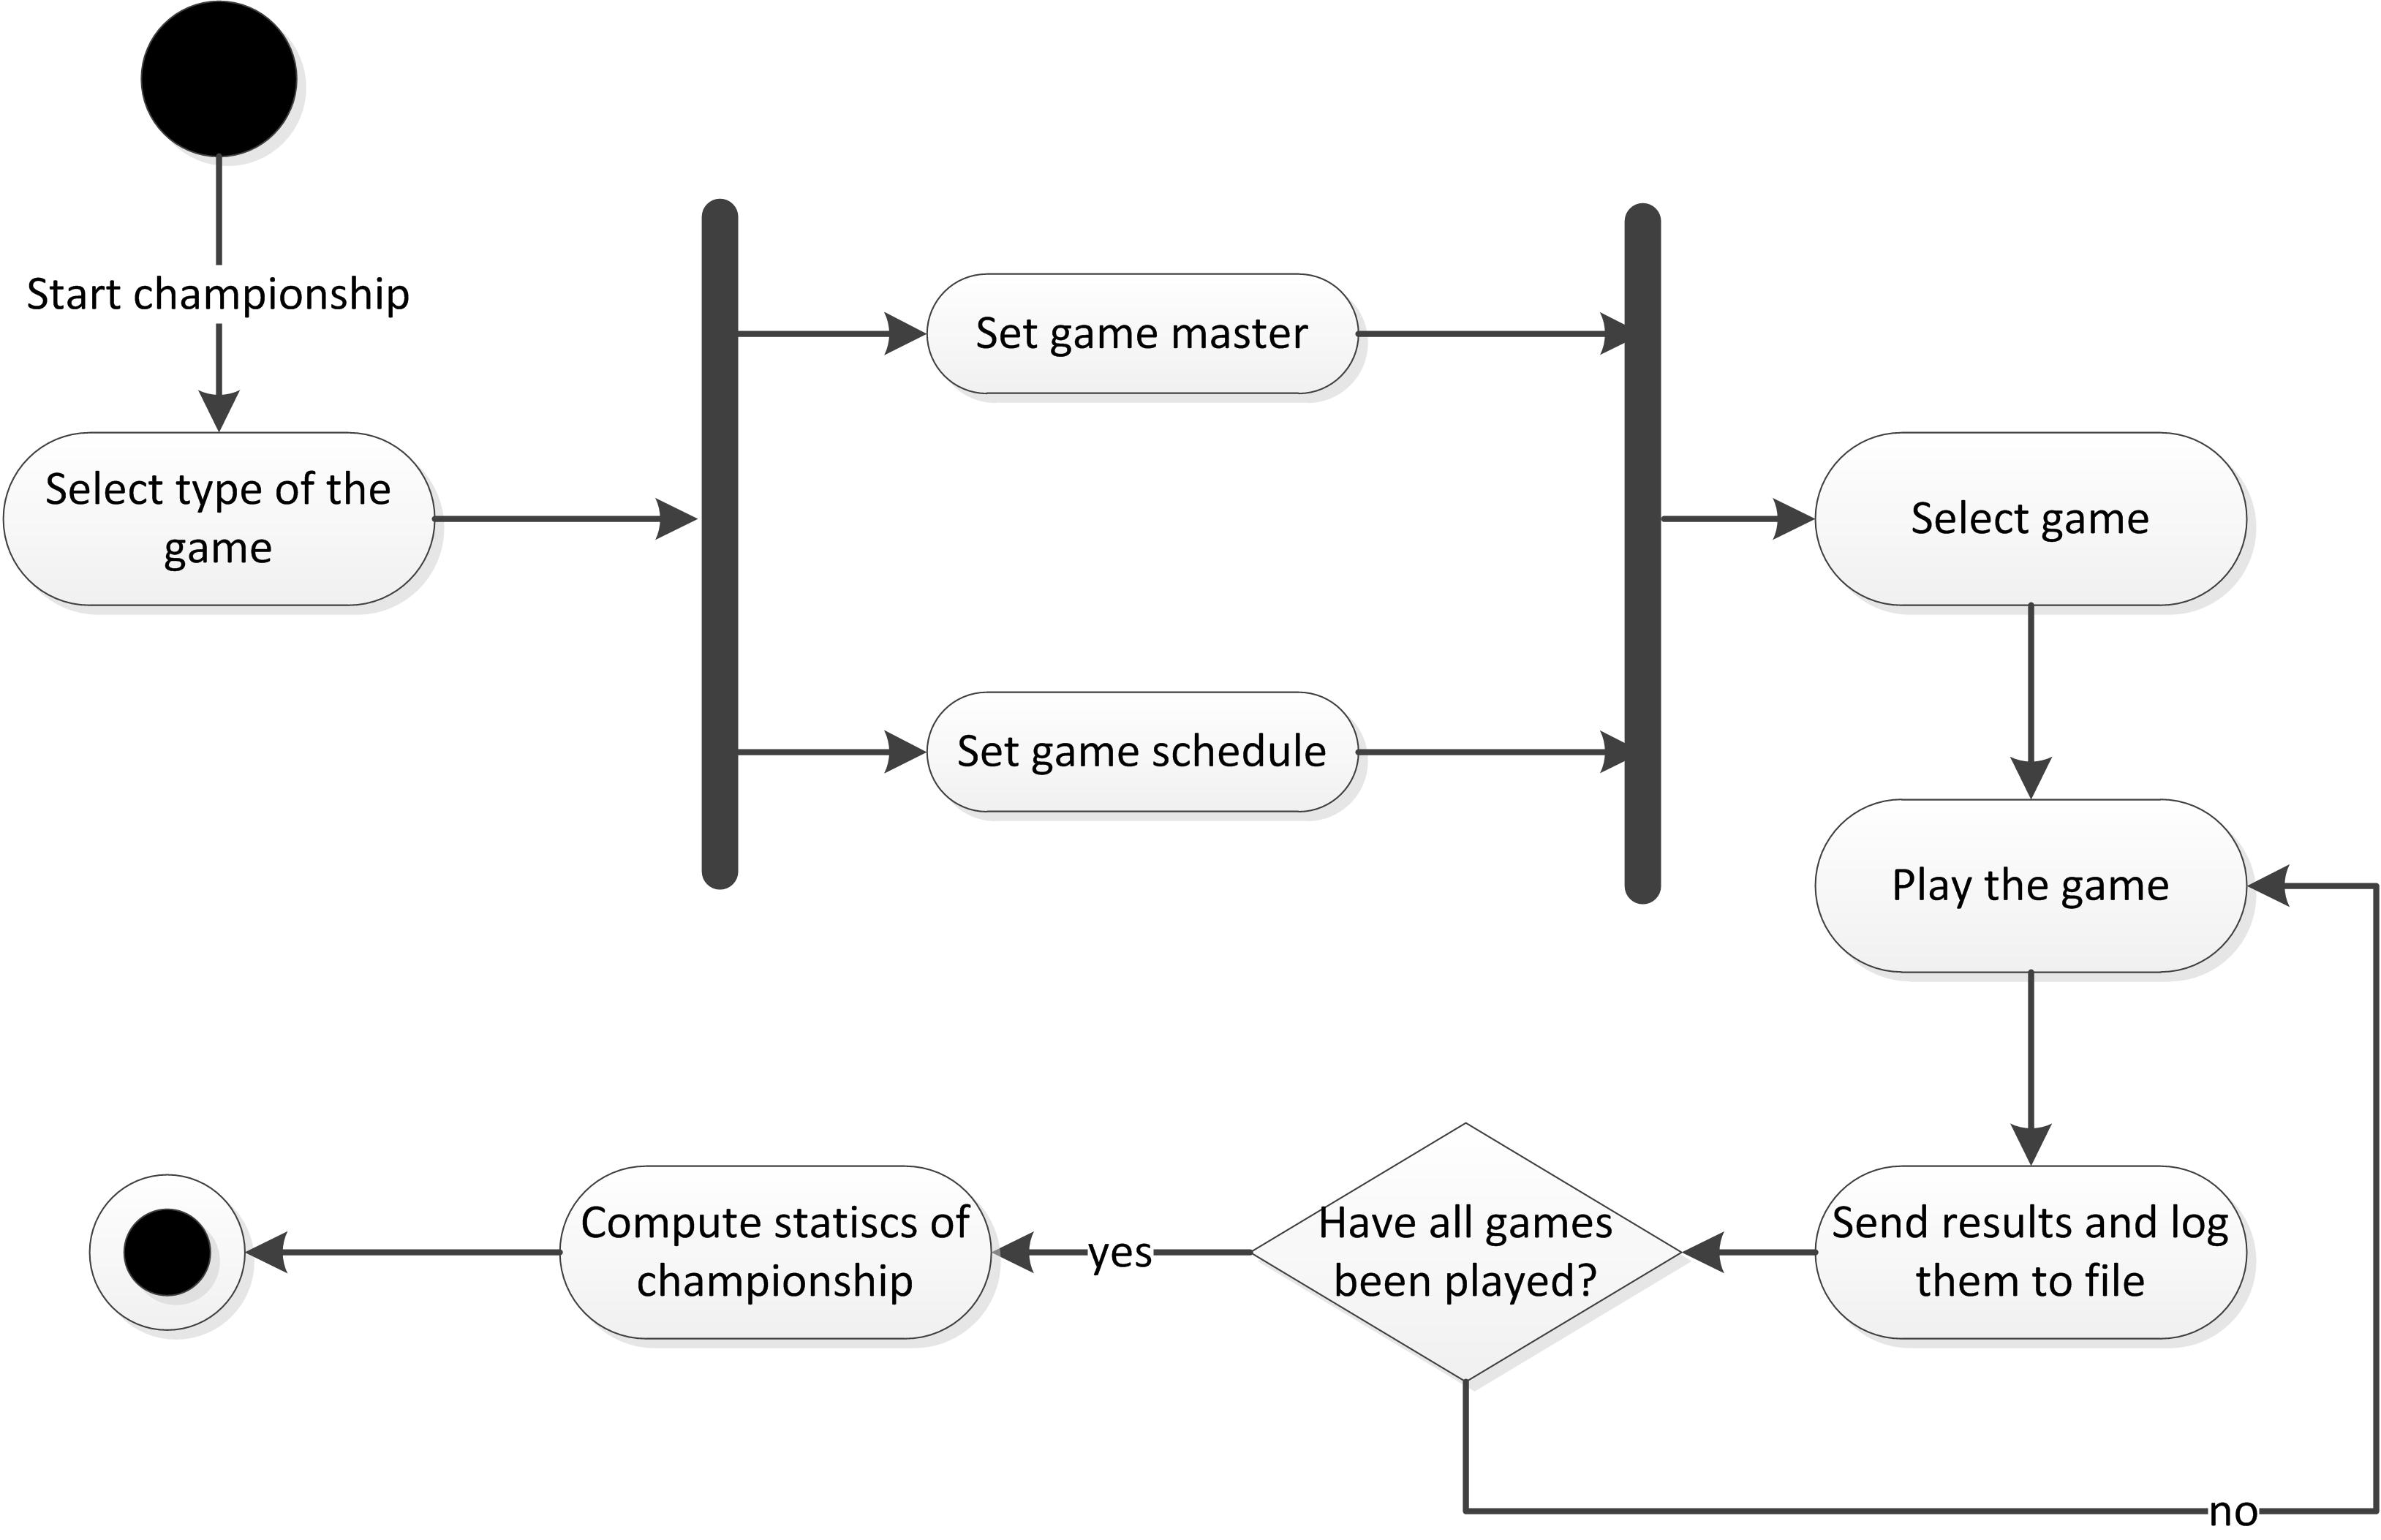
\includegraphics[scale=0.80]{UGS_activities_champioship_management.jpg}


\pagebreak[4]


\subsection{Game creation}
Both server and game master participate in the process of game creation.

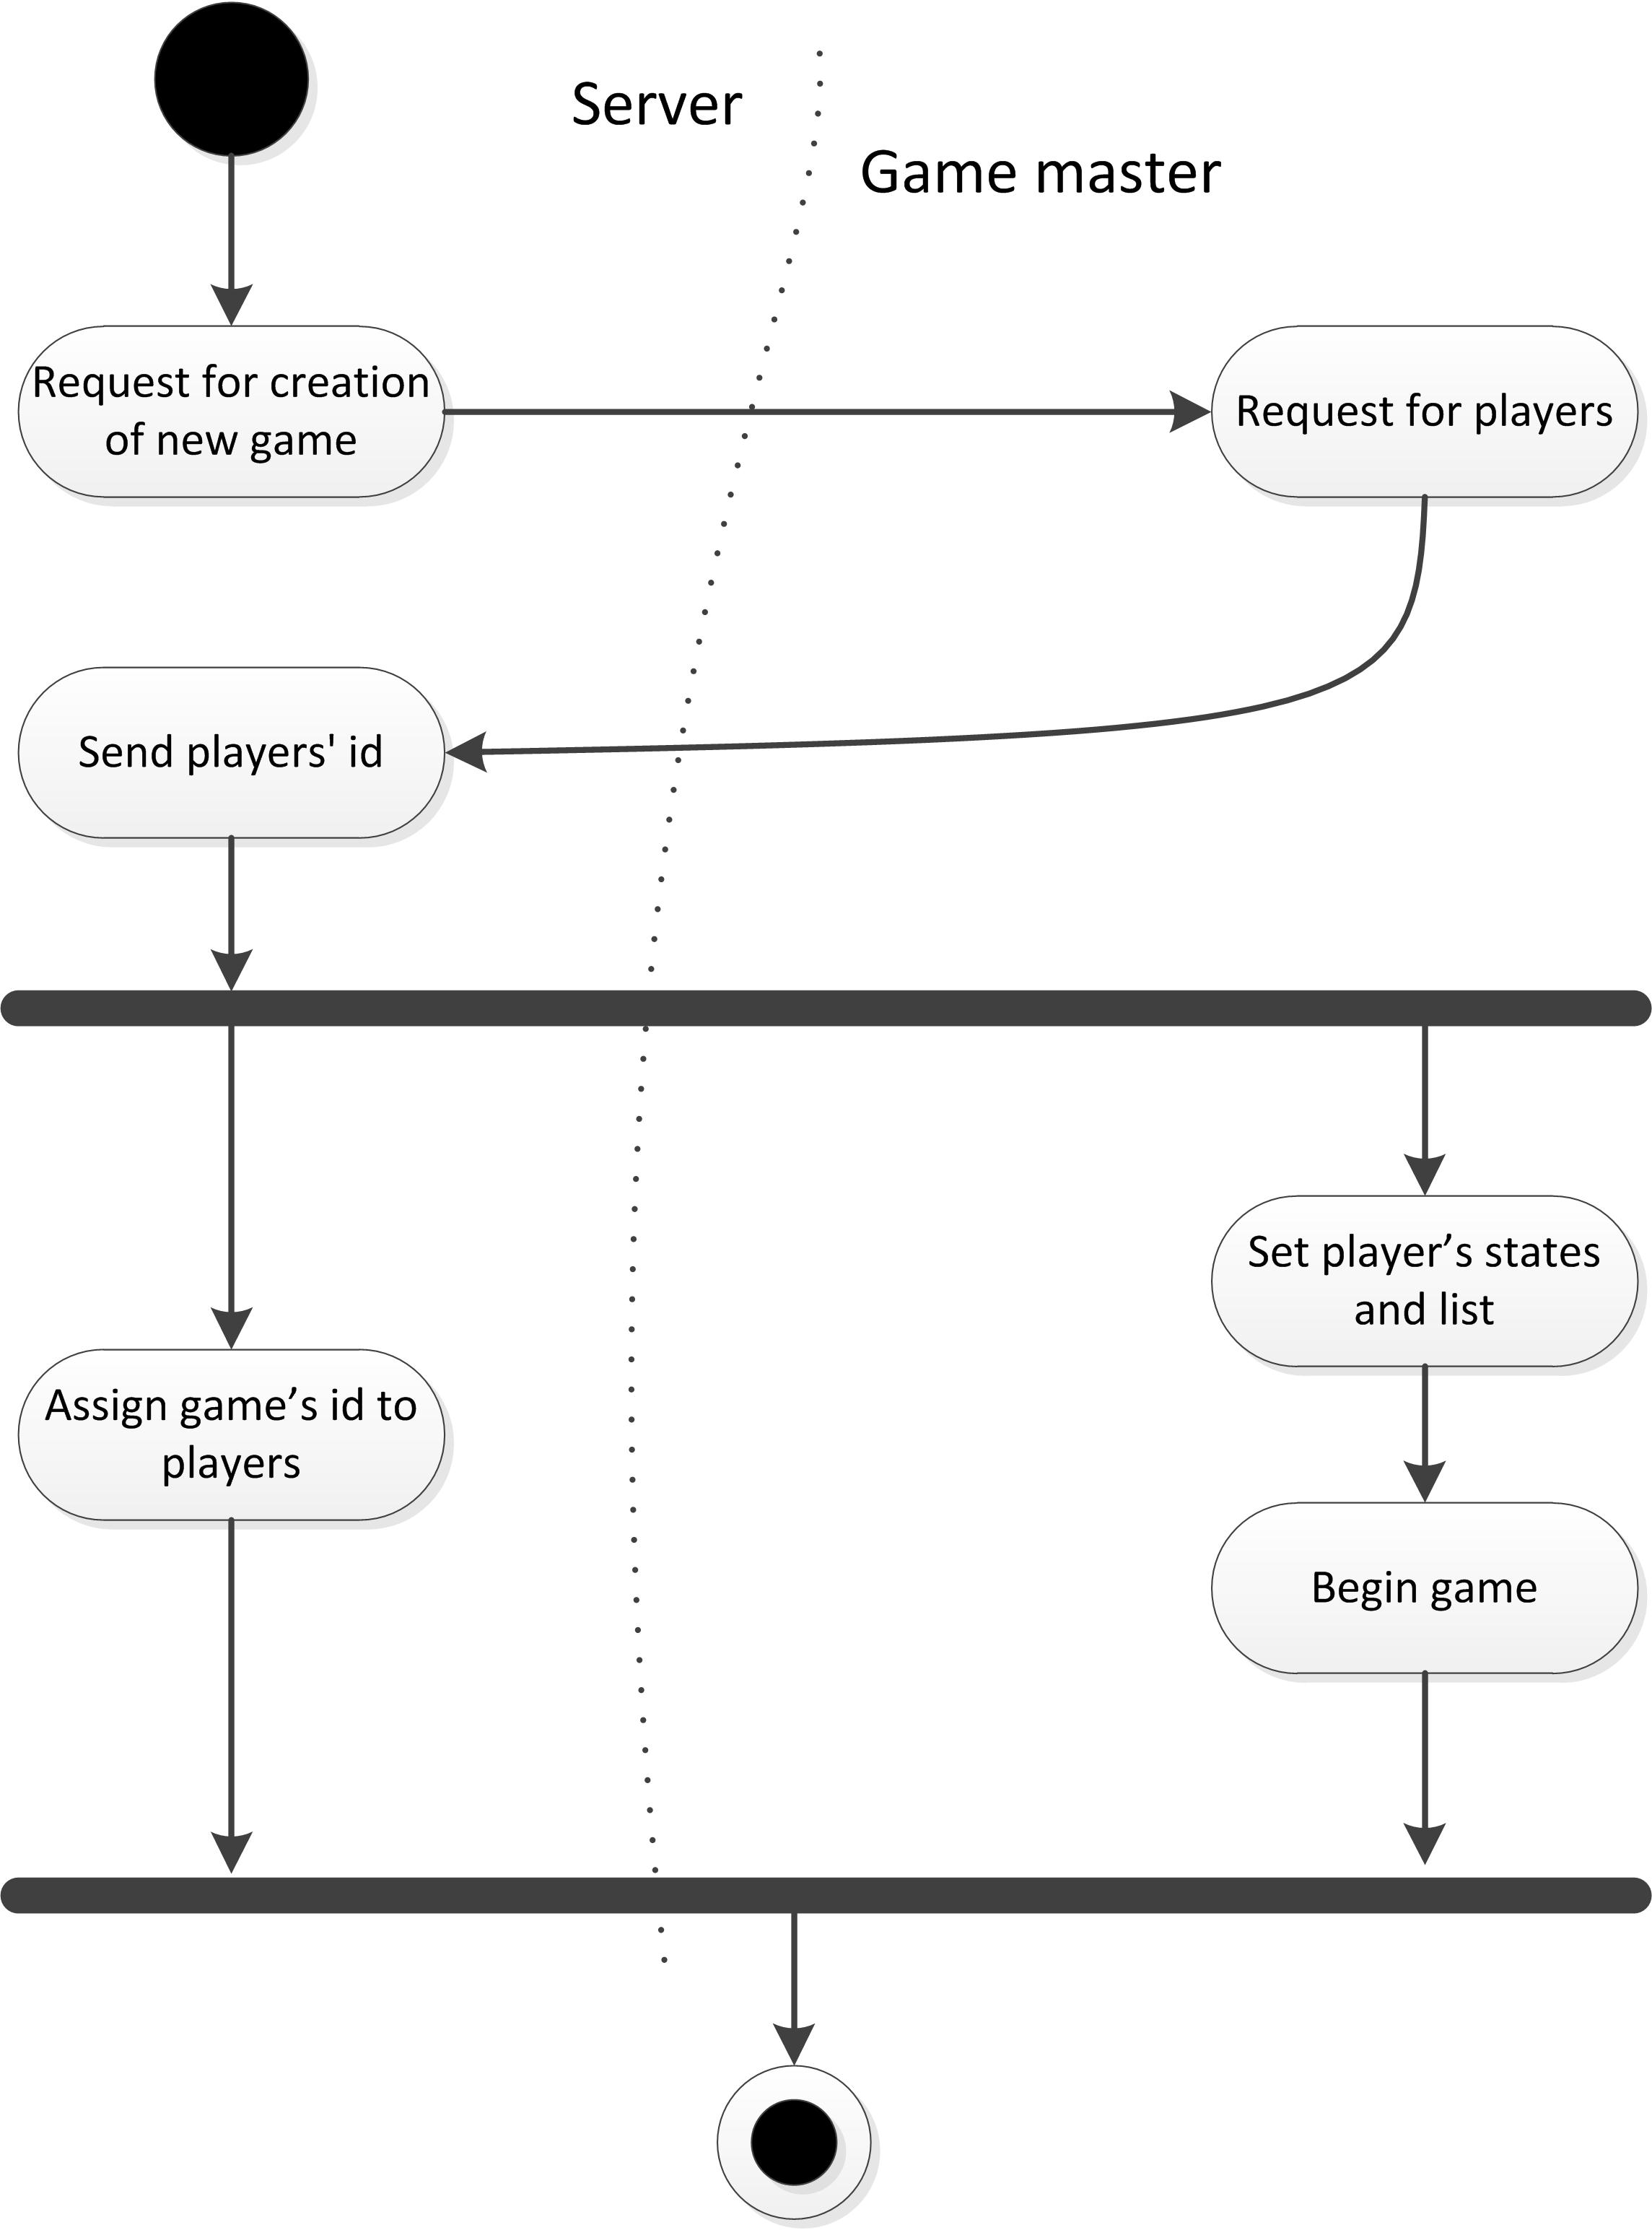
\includegraphics[scale=1.00]{UGS_activities_game_creation.jpg}

\subsection{Login}
The below diagram shows the procedure of adding a client to a server.

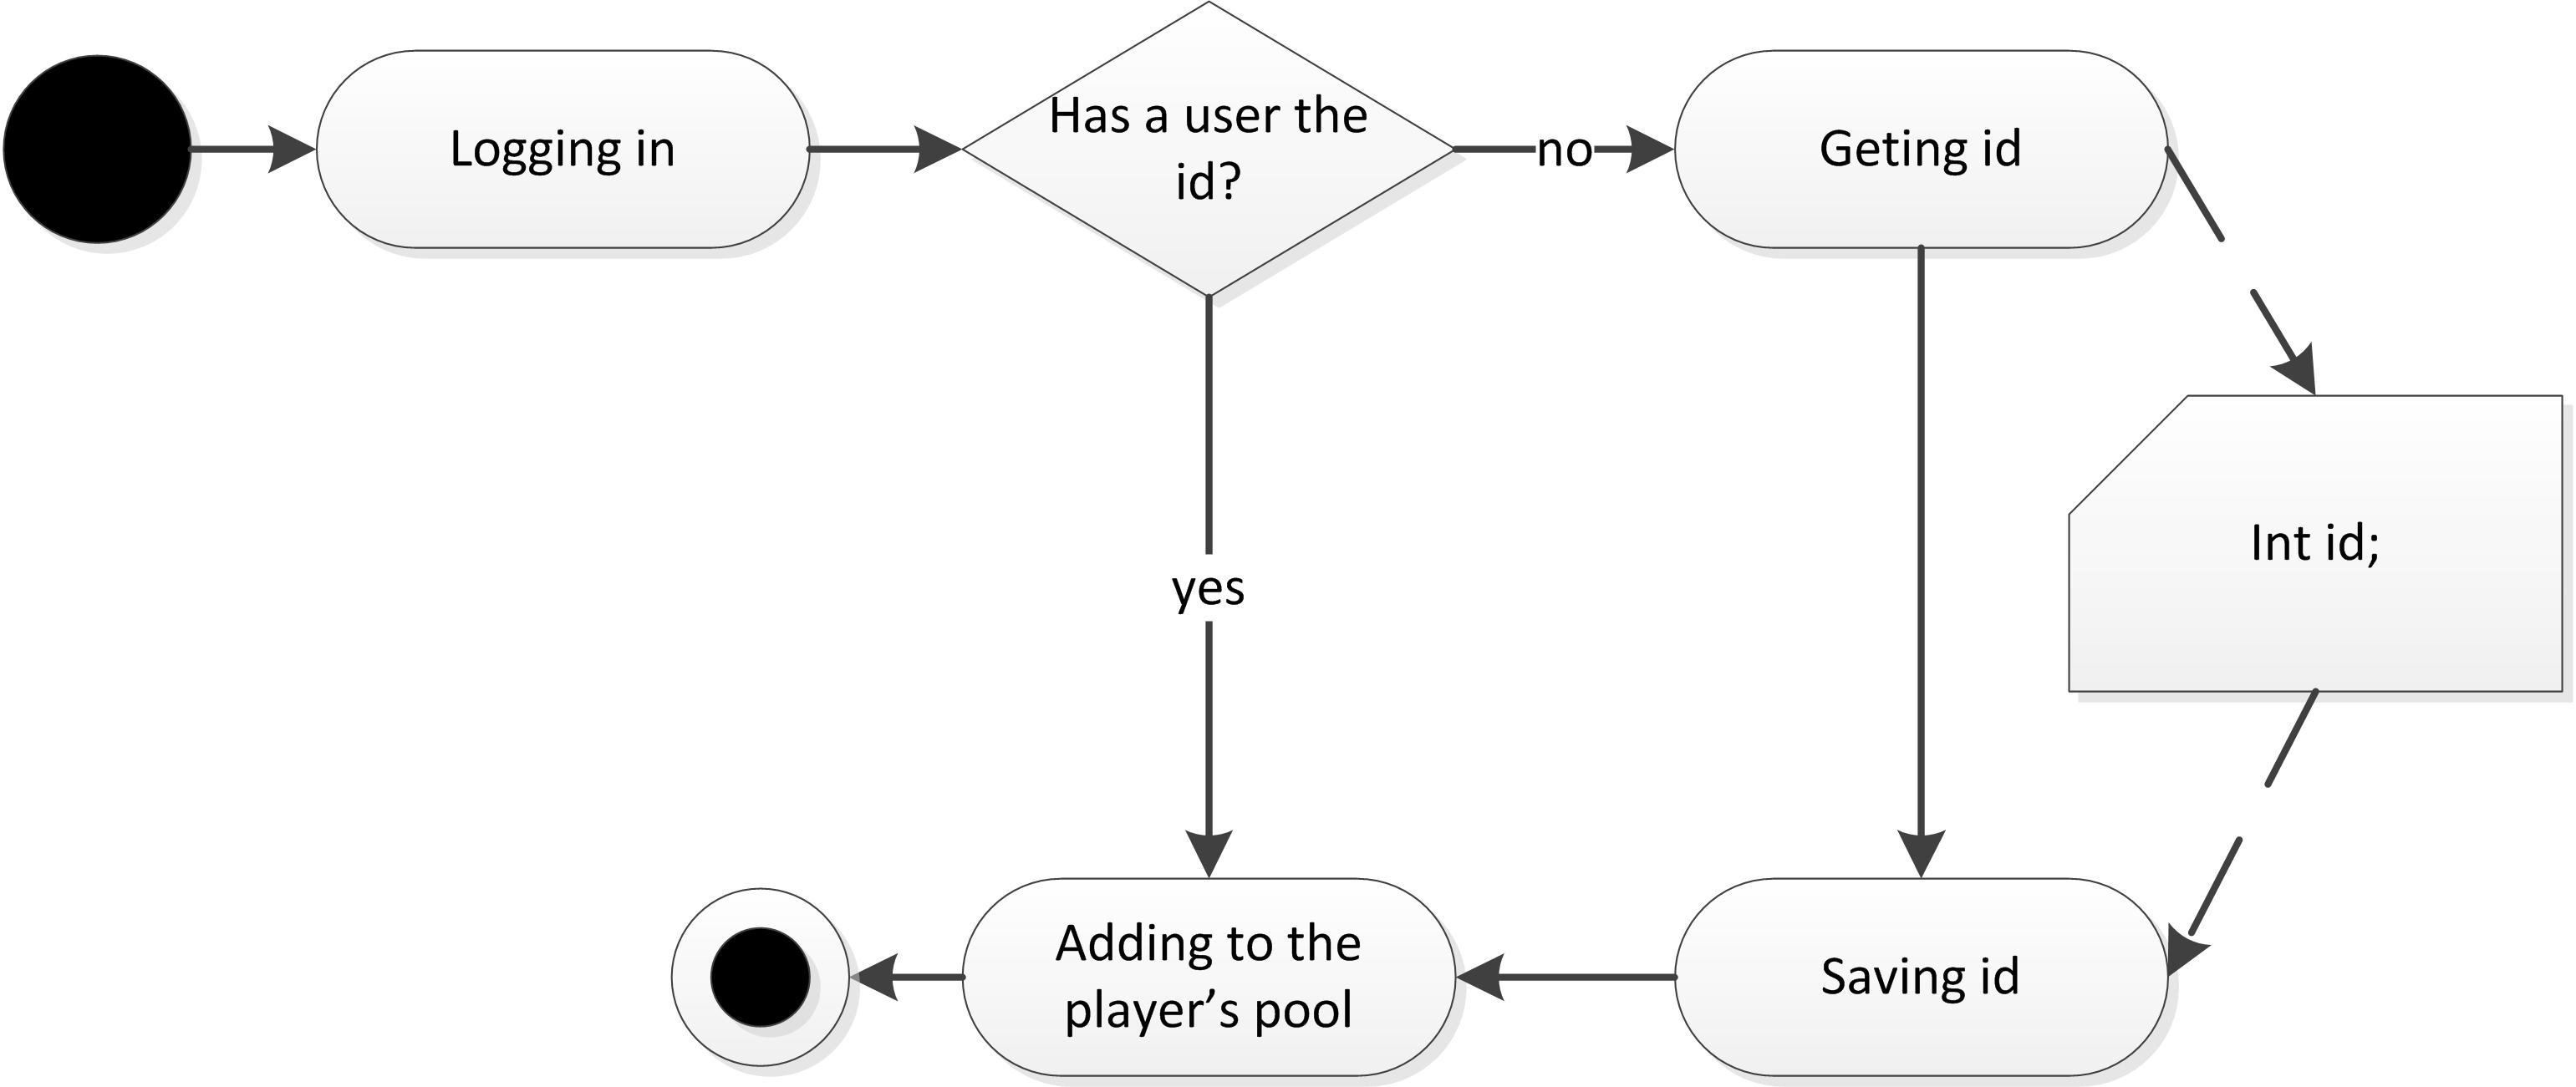
\includegraphics[scale=1.00]{UGS_activities_login.jpg}


\pagebreak[4]


\subsection{Logout}
Below diagram depicts the process of removing the client from the server.

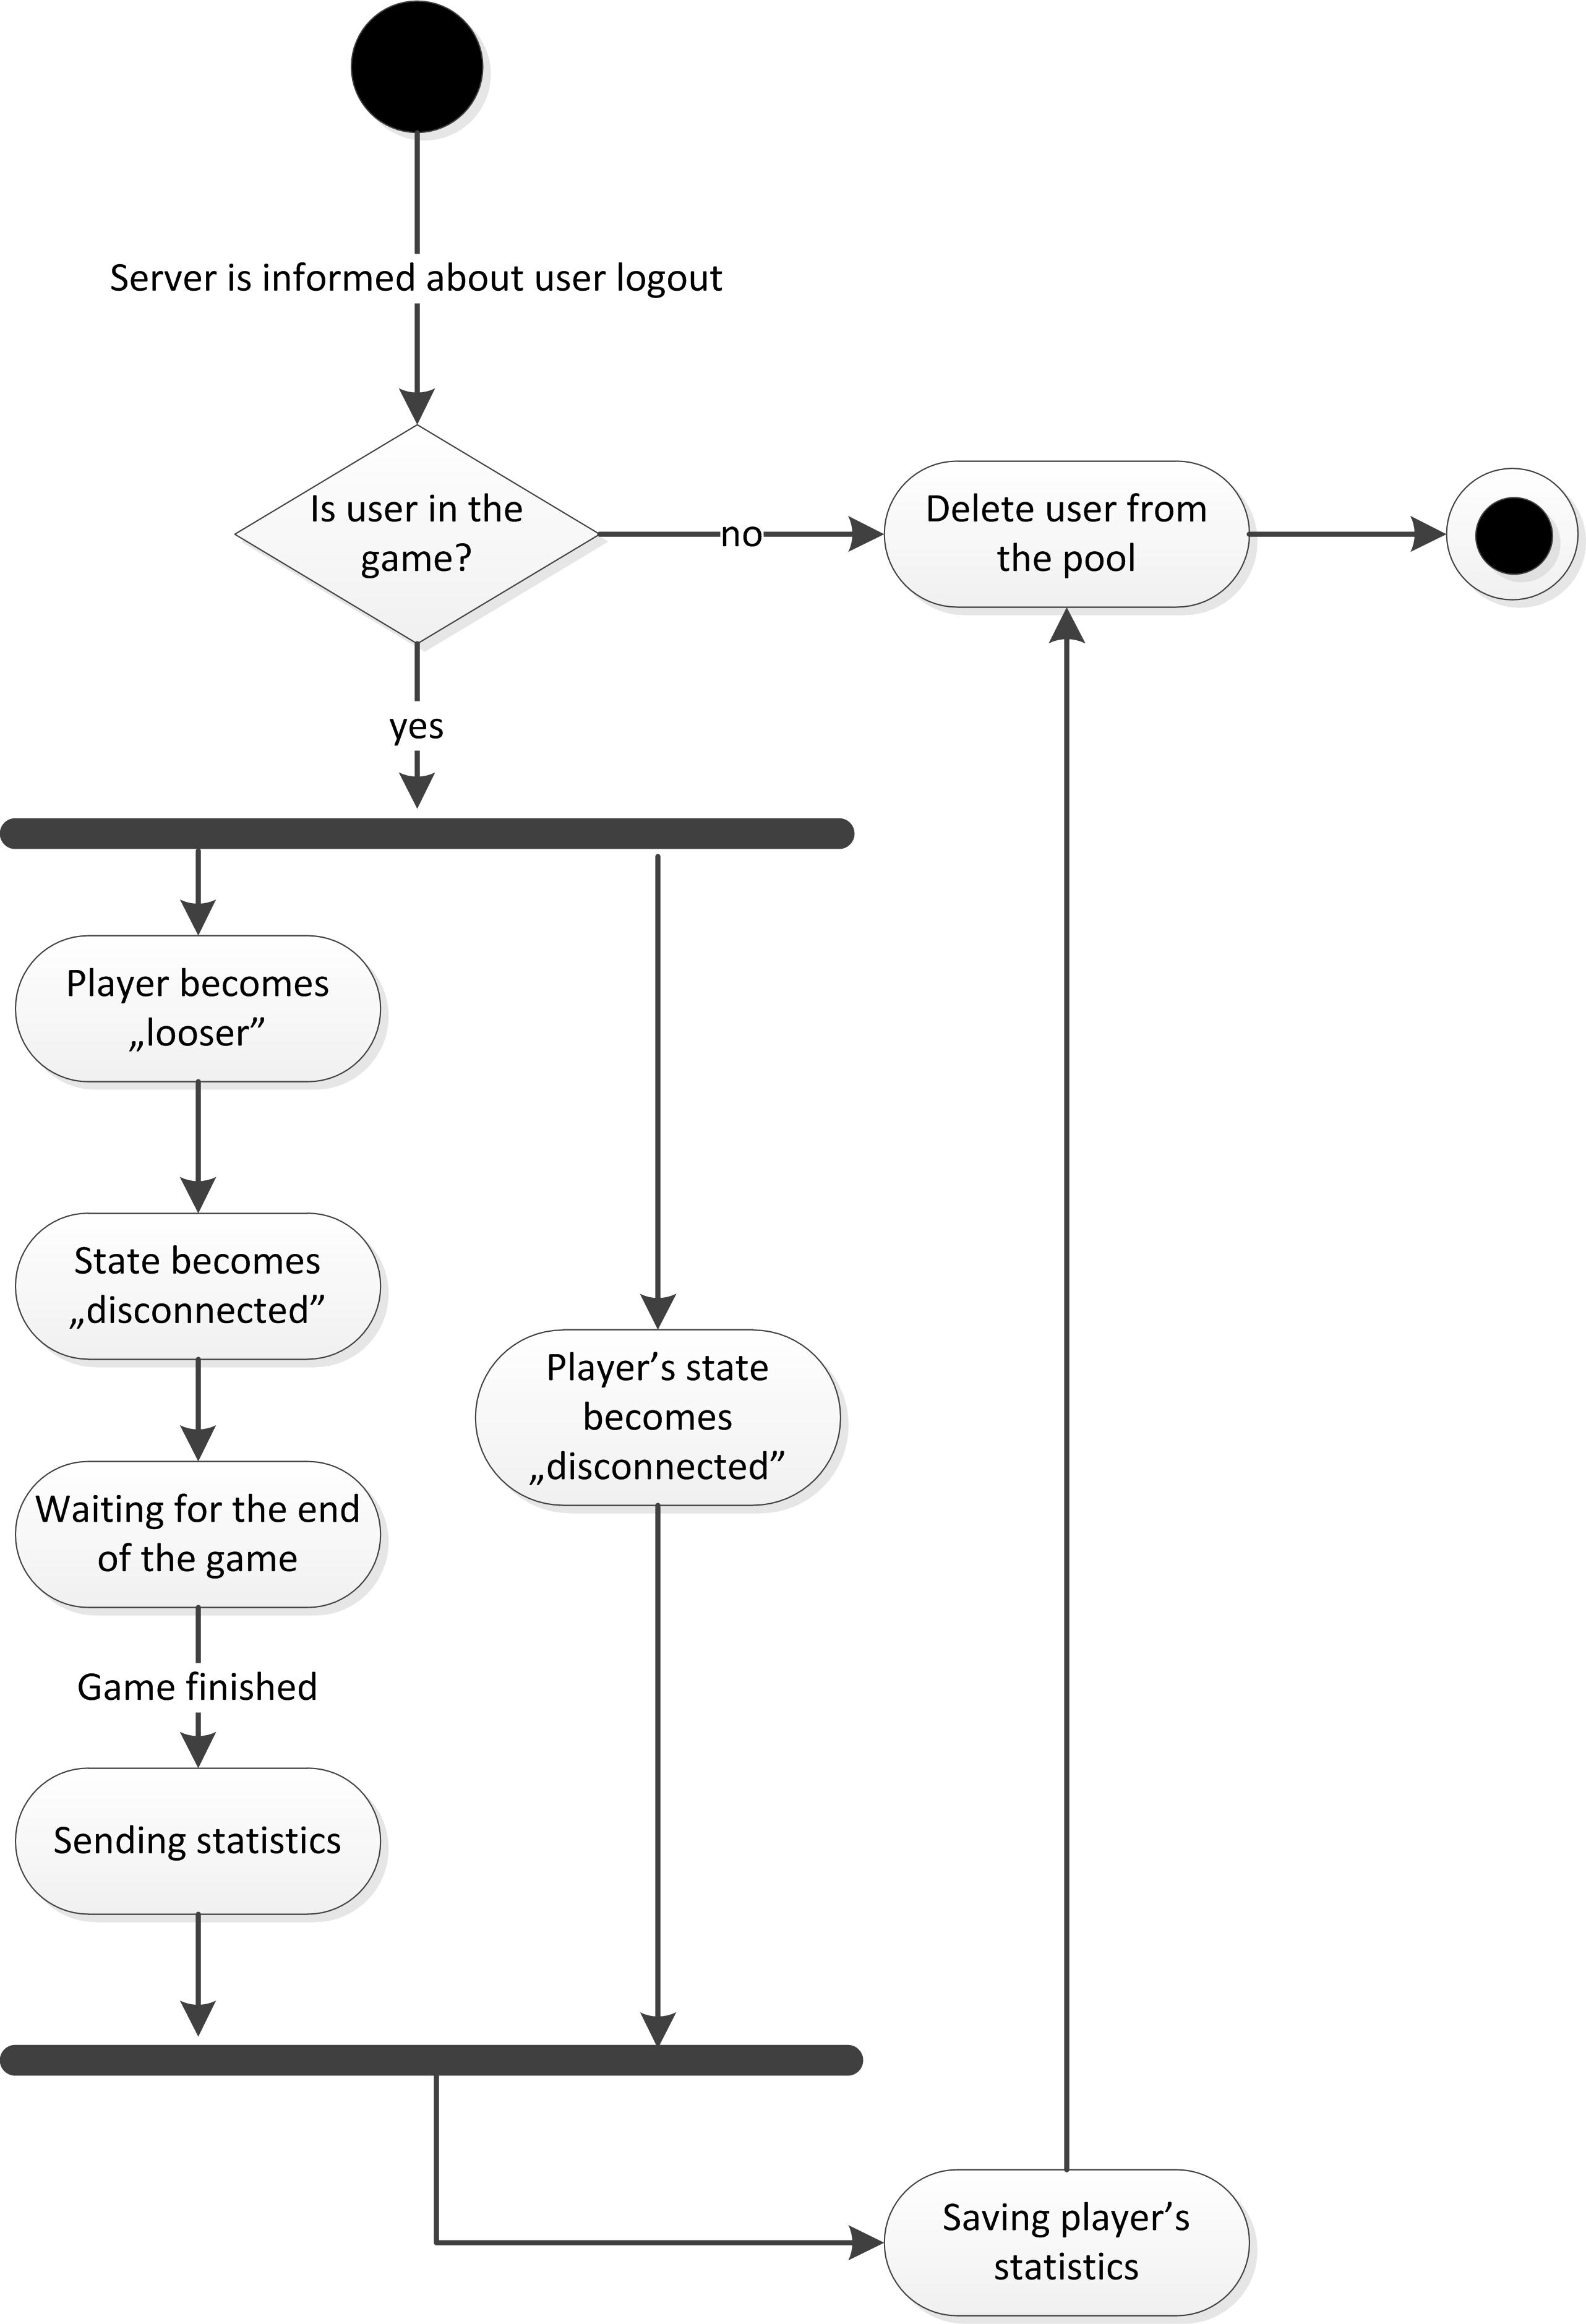
\includegraphics[scale=1.00]{UGS_activities_logout.jpg}

\section{Additional comments}
\begin{itemize}
  \item Universal Game System is designed to organize games between game applications.
  \item It consists of three applications working together: game player, game master and game server.
  \item Master and Player application supports timeout and illegal movement detection.
  \item The server is the only connection between game masters and players.
  \item All players work in a loop.
  \item Game termination messages are handled in a different way depending on what is the reason of termination.
  \item All application should support handling termination messages.
\end{itemize}

\end{document}
